%%%%%%%%%%%%%%%%%%%%%%%%%%%%%%%%%%%%%%%%%%%%%%%%%%%
%
%  New template code for TAMU Theses and Dissertations starting Fall 2012.  
%  For more info about this template or the 
%  TAMU LaTeX User's Group, see http://www.howdy.me/.
%
%  Author: Wendy Lynn Turner 
%
%%%%%%%%%%%%%%%%%%%%%%%%%%%%%%%%%%%%%%%%%%%%%%%%%%%

\documentclass[12pt]{report}
\usepackage[letterpaper]{geometry}
\geometry{verbose,tmargin=1.25in,bmargin=1.25in,lmargin=1.4in,rmargin=1.15in}
 \usepackage[doublespacing]{setspace}
 \usepackage{tocloft}
 \usepackage[rm, tiny,center, compact]{titlesec}
 \usepackage{indentfirst}
 \usepackage{etoolbox}
\usepackage{tocvsec2}
 \usepackage[titletoc]{appendix}
 \usepackage{appendix}
 \usepackage{tamuconfig}
\usepackage{rotating}
\usepackage{float}

% Added to fix issues with pdf searching in some versions of LaTeX
%\usepackage[T1]{fontenc}\usepackage{lmodern}
%%%%%%%%%%%%%%%%%%%%%%%%%%%%%

% Hyperref setup below.  You should be able to get away with using uncommenting just the first line.
%\usepackage[hidelinks]{hyperref}

% if \usepackage[hidelinks]{hyperref} doesn't work try this.
% \usepackage{hyperref}  % Hidelinks is an option that removes link visiability.  TAMU Thesis Offices prefers to not see the links. But often doesn't work.  
% 
% \hypersetup{
%     colorlinks=true,
%     linkcolor=black,
%     citecolor=black,
%     filecolor=black,
%     urlcolor=black,
% }
%%%%%%%  End of hyperref setup.  One of these two options should work, but my motto with hyperref is when in doubt, comment it out!
%%%%%%%%%  This hopefully fixes the problem with vertical spacing of section headings at the top of the page..  Commented out in 1.0.7
% \preto\section{%
% \ifnum\value{section}>0\addtocontents{toc}{\vskip-6pt}\fi
% }
% \preto\subsection{%
% \ifnum\value{subsection}=0\addtocontents{toc}{\vskip-6pt}\fi
% \ifnum\value{subsection}>0\addtocontents{toc}{\vskip-6pt}\fi
% } 
%%%%%%%%%%%%%%%%%%%%%%%%%%%%%%%%%%%%%%%%%%%%%%%%%%%%%%

\begin{document}

\renewcommand{\tamumanuscripttitle}{Load Balancing Unstructured Meshes for Massively Parallel Transport Sweeps}
\renewcommand{\tamupapertype}{Thesis}
\renewcommand{\tamufullname}{Tarek Habib Ghaddar}
\renewcommand{\tamudegree}{Master of Science}
\renewcommand{\tamuchairone}{Dr. Jean Ragusa}
% Uncomment out the next line if you have co-chairs.  You will also need to edit the titlepage.tex file.
%\newcommand{\tamuchairtwo}{Additional Chair Name}
\renewcommand{\tamumemberone}{Dr. Jim Morel}
\newcommand{\tamumembertwo}{Dr. Bojan Popov}
\newcommand{\tamumemberthree}{Committee Member3}
\renewcommand{\tamudepthead}{Dr. Yassin Hassan}
\renewcommand{\tamugradmonth}{May}
\renewcommand{\tamugradyear}{2016}
\renewcommand{\tamudepartment}{Nuclear Engineering}


%%%%%%%%%%%%%%%%%%%%%%%%%%%%%%%%%%%%%%%%%%%%%%%%%%%
%
%  New template code for TAMU Theses and Dissertations starting Fall 2012.  
%  For more info about this template or the 
%  TAMU LaTeX User's Group, see http://www.howdy.me/.
%
%  Author: Wendy Lynn Turner 
%	 Version 1.0 
%  Last updated 8/5/2012
%
%%%%%%%%%%%%%%%%%%%%%%%%%%%%%%%%%%%%%%%%%%%%%%%%%%%

%%%%%%%%%%%%%%%%%%%%%%%%%%%%%% 
%% TITLE PAGE
%% The values get updated automatically.  Please do not make changes to this file other than adding/deleting committee members where necessary.
%%%%%%%%%%%%%%%%%%%%%%%%%%%%%%

\providecommand{\tabularnewline}{\\}



\begin{titlepage}
\begin{center}
\MakeUppercase{\tamumanuscripttitle}
\vspace{4em}

A \tamupapertype

by

\MakeUppercase{\tamufullname}

\vspace{4em}

\begin{singlespace}

Submitted to the Office of Graduate and Professional Studies of \\
Texas A\&M University \\

in partial fulfillment of the requirements for the degree of \\
\end{singlespace}

\MakeUppercase{\tamudegree}
\par\end{center}
\vspace{2em}
\begin{singlespace}
\begin{tabular}{ll}
 & \tabularnewline
& \cr
% If you have Co-Chairs comment out the 'Chair of Committee' line below and uncomment the 'Co-Chairs of Committee' line.
Chair of Committee, & \tamuchairone\tabularnewline
%Co-Chairs of Committee, & \tamuchairone\tabularnewline & \tamuchairtwo\tabularnewline
Committee Members, & \tamumemberone\tabularnewline
 & \tamumembertwo\tabularnewline
Head of Department, & \tamudepthead\tabularnewline

\end{tabular}
\end{singlespace}
\vspace{3em}

\begin{center}
\tamugradmonth \hspace{2pt} \tamugradyear

\vspace{3em}

Major Subject: \tamudepartment \par
\vspace{3em}
Copyright \tamugradyear \hspace{.5em}\tamufullname 
\par\end{center}
\end{titlepage}
\pagebreak{}




 % This is simply a file that formats and adds your titlepage, please do not edit this unless you have a specific need. .
%%%%%%%%%%%%%%%%%%%%%%%%%%%%%%%%%%%%%%%%%%%%%%%%%%%
%
%  New template code for TAMU Theses and Dissertations starting Fall 2016.  
%
%
%  Author: Sean Zachary Roberson
%  Version 3.17.09
%  Last Updated: 9/21/2017
%
%%%%%%%%%%%%%%%%%%%%%%%%%%%%%%%%%%%%%%%%%%%%%%%%%%%
%%%%%%%%%%%%%%%%%%%%%%%%%%%%%%%%%%%%%%%%%%%%%%%%%%%%%%%%%%%%%%%%%%%%%
%%                           ABSTRACT 
%%%%%%%%%%%%%%%%%%%%%%%%%%%%%%%%%%%%%%%%%%%%%%%%%%%%%%%%%%%%%%%%%%%%%

\chapter*{ABSTRACT}
\addcontentsline{toc}{chapter}{ABSTRACT} % Needs to be set to part, so the TOC doesnt add 'CHAPTER ' prefix in the TOC.

\pagestyle{plain} % No headers, just page numbers
\pagenumbering{roman} % Roman numerals
\setcounter{page}{2}

\indent The field of radiation transport studies the distribution of radiation throughout a seven-dimensional phase-space consisting of time, space, energy, and direction. Radiation transport is described by the Boltzmann equation and can be solved stochastically or deterministically.

The work presented in this dissertation utilizes the deterministic method known as the transport sweep, a popular technique that has been the subject of a large amount of research.
We specifically focus on the parallel implementations of the transport sweep, and predicting the time it takes to sweep across a structured or unstructured mesh given a set of partitioning parameters, achieved through a time-to-solution estimator, written in Python.
The time-to-solution estimator is tested against PDT, Texas A\&M's massively deterministic transport code.
The time-to-solution estimator's sweep time is within 10\% of PDT's sweep time for the majority of problems tested.

We use the time-to-solution estimator as the objective function in an optimization scheme to attempt to get the partitions that lead to the fastest sweep time for a given problem and partitioning scheme.
Two optimization methods are discussed: using a black box tool (scipy's optimize library) and an intuitive method that relies on placing partitions in mesh locations that does not increase the number of cells (which we chose to name the CDF method).
The time-to-solution estimator proved to not be smooth enough for a black box tool to work, so the geometry based optimization method became the primary method.
The CDF method proved effective for our unbalanced pin test problem, improving the time to solution over previously used partitioning schemes.
For our larger test problem, the optimized partitioning scheme improves the time to solution over one previously used partitioning scheme, but is not as effective relative to other previously used partitioning schemes.
\pagebreak{}

%%%%%%%%%%%%%%%%%%%%%%%%%%%%%%%%%%%%%%%%%%%%%%%%%%%
%
%  New template code for TAMU Theses and Dissertations starting Fall 2016.  
%
%
%  Author: Sean Zachary Roberson
%  Version 3.17.09
%  Last Updated: 9/21/2017
%
%%%%%%%%%%%%%%%%%%%%%%%%%%%%%%%%%%%%%%%%%%%%%%%%%%%

%%%%%%%%%%%%%%%%%%%%%%%%%%%%%%%%%%%%%%%%%%%%%%%%%%%%%%%%%%%%%%%%%%%%%%
%%                           DEDICATION
%%%%%%%%%%%%%%%%%%%%%%%%%%%%%%%%%%%%%%%%%%%%%%%%%%%%%%%%%%%%%%%%%%%%%
\chapter*{DEDICATION}
\addcontentsline{toc}{chapter}{DEDICATION}  % Needs to be set to part, so the TOC doesnt add 'CHAPTER ' prefix in the TOC.



\begin{center}
\vspace*{\fill}
To my mother, my father, my grandfather, and my grandmother. To see what happens with multiple lines, I extend this next part into a second line.
\vspace*{\fill}
\end{center}

\pagebreak{}

%%%%%%%%%%%%%%%%%%%%%%%%%%%%%%%%%%%%%%%%%%%%%%%%%%%
%
%  New template code for TAMU Theses and Dissertations starting Fall 2016.  
%
%
%  Author: Sean Zachary Roberson
%  Version 3.17.09
%  Last Updated: 9/21/2017
%
%%%%%%%%%%%%%%%%%%%%%%%%%%%%%%%%%%%%%%%%%%%%%%%%%%%


%%%%%%%%%%%%%%%%%%%%%%%%%%%%%%%%%%%%%%%%%%%%%%%%%%%%%%%%%%%%%%%%%%%%%%
%%                           ACKNOWLEDGMENTS
%%%%%%%%%%%%%%%%%%%%%%%%%%%%%%%%%%%%%%%%%%%%%%%%%%%%%%%%%%%%%%%%%%%%%
\chapter*{ACKNOWLEDGMENTS}
\addcontentsline{toc}{chapter}{ACKNOWLEDGMENTS}  % Needs to be set to part, so the TOC doesnt add 'CHAPTER ' prefix in the TOC.


\indent I would like to thank Dr. Jean Ragusa for toeing the line between demanding and understanding perfectly. I know I haven't made your job as my advisor easy. 

Thank you to my committee, Drs. Adams, Amato, and Morel, for the feedback and advice when needed to push this work to completion.

A special thank you to Daryl Hawkins, a man I'm convinced is the most overworked code developer on the planet. This work would have been impossible without him. 

Thank you to Andrew Till for always being a sounding board for academic ideas, and thank you to Ian Halvic for dealing with my less than fine moments in the office. 

Thank you to Dillon Herring for his accelerated effort on his Master's project, which helped the completion of this dissertation.

To Nicolas Quintanar, Brian Ng, and David Saucier, thank you for keeping my life fun and full of life. 

To the CERT team, thank you for your constant support in all of my research endeavors.




\pagebreak{}
%%%%%%%%%%%%%%%%%%%%%%%%%%%%%%%%%%%%%%%%%%%%%%%%%%%
%
%  New template code for TAMU Theses and Dissertations starting Fall 2012.  
%  For more info about this template or the 
%  TAMU LaTeX User's Group, see http://www.howdy.me/.
%
%  Author: Wendy Lynn Turner 
%	 Version 1.0 
%  Last updated 8/5/2012
%
%%%%%%%%%%%%%%%%%%%%%%%%%%%%%%%%%%%%%%%%%%%%%%%%%%%

%%%%%%%%%%%%%%%%%%%%%%%%%%%%%%%%%%%%%%%%%%%%%%%%%%%%%%%%%%%%%%%%%%%%%%
%%                           NOMENCLATURE
%%%%%%%%%%%%%%%%%%%%%%%%%%%%%%%%%%%%%%%%%%%%%%%%%%%%%%%%%%%%%%%%%%%%%

\chapter*{NOMENCLATURE}
\addcontentsline{toc}{chapter}{NOMENCLATURE}  % Needs to be set to part, so the TOC doesnt add 'CHAPTER ' prefix in the TOC.

\begin{tabular}{ll}
B/CS  & Bryan/College Station\tabularnewline
HSUS & Humane Society of the United States\tabularnewline
P & Pressure\tabularnewline
T  & Time\tabularnewline
TVA & Tennessee Valley Authority\tabularnewline
TxDOT \hfill{}\hfill{}\hfill{}\hfill{}\hfill{}\hfill{}\hfill{}\hfill{} & \multicolumn{1}{l}{Texas Department of Transportation}\tabularnewline
\end{tabular}

\vspace{2em}

This page is optional.

\pagebreak{}

%%%%%%%%%%%%%%%%%%%%%%%%%%%%%%%%%%%%%%%%%%%%%%%%%%%
%
%  New template code for TAMU Theses and Dissertations starting Fall 2012.  
%  For more info about this template or the 
%  TAMU LaTeX User's Group, see http://www.howdy.me/.
%
%  Author: Wendy Lynn Turner 
%	 Version 1.7
%  Last updated 3/24/2014
%
%%%%%%%%%%%%%%%%%%%%%%%%%%%%%%%%%%%%%%%%%%%%%%%%%%%
%%%%%%%%%%%%%%%%%%%%%%%%%%%%%%%%%%%%%%%%%%%%%%%%%%%%%%%%%%%%%%%%%%%%%%
%%       TABLE OF CONTENTS
%%%%%%%%%%%%%%%%%%%%%%%%%%%%%%%%%%%%%%%%%%%%%%%%%%%%%%%%%%%%%%%%%%%%%
% single-space sections in Table of Contents  - commented in version 1.7
%\renewcommand{\cftsecafterpnum}{\vskip0.5\baselineskip}
%\renewcommand{\cftsubsecafterpnum}{\vskip0.5\baselineskip}
%\renewcommand{\cftsubsubsecafterpnum}{\vskip0.5\baselineskip}
%%%%%%%%%%%%%%%%%%%%%%%%%%%%%%%%%%%%%%%%%%%%%%%%%%%

\phantomsection
\addcontentsline{toc}{chapter}{TABLE OF CONTENTS}  

\begin{singlespace}
\renewcommand\contentsname{\normalfont} {\centerline{TABLE OF CONTENTS}}

%\setcounter{tocdepth}{4} % This puts \subsubsection[]{×} in your List of Tables.  The default is 3.


%%%%%%%%%%%%%  Adds Page above the page number in TOC
\setlength{\cftaftertoctitleskip}{1em}
\renewcommand{\cftaftertoctitle}{%
\hfill{\normalfont {Page}\par}}



\tableofcontents

\end{singlespace}

\pagebreak{}

%%%%%%%%%%%%%%%%%%%%%%%%%%%%%%%%%%%%%%%%%%%%%%%%%%%%%%%%%%%%%%%%%%%%%%
%%                           LIST OF FIGURES
%%%%%%%%%%%%%%%%%%%%%%%%%%%%%%%%%%%%%%%%%%%%%%%%%%%%%%%%%%%%%%%%%%%%%

\phantomsection
\addcontentsline{toc}{chapter}{LIST OF FIGURES}  

\renewcommand{\cftloftitlefont}{\center\normalfont\MakeUppercase}

\setlength{\cftbeforeloftitleskip}{-12pt} %% Positions the LOF title vertically to match the chapter titles
\renewcommand{\cftafterloftitleskip}{12pt}


\renewcommand{\cftafterloftitle}{%
\\[4em]\mbox{}\hspace{2pt}FIGURE\hfill{\normalfont Page}\vskip\baselineskip}

\begingroup


\begin{center}
\begin{singlespace}
%% These values make the lof table entries appear double spaced between.
\setlength{\cftbeforechapskip}{0.4cm}
\setlength{\cftbeforesecskip}{0.30cm}
\setlength{\cftbeforesubsecskip}{0.30cm}
\setlength{\cftbeforefigskip}{0.4cm}
\setlength{\cftbeforetabskip}{0.4cm} 

\listoffigures

\end{singlespace}
\end{center}

\pagebreak{}


%%%%%%%%%%%%%%%%%%%%%%%%%%%%%%%%%%%%%%%%%%%%%%%%%%%%%%%%%%%%%%%%%%%%%%
%%                           lIST OF TABLES
%%%%%%%%%%%%%%%%%%%%%%%%%%%%%%%%%%%%%%%%%%%%%%%%%%%%%%%%%%%%%%%%%%%%%%
%
\phantomsection
\addcontentsline{toc}{chapter}{LIST OF TABLES}  

\renewcommand{\cftlottitlefont}{\center\normalfont\MakeUppercase}

\setlength{\cftbeforelottitleskip}{-12pt} %% Positions the LOT title vertically to match the chapter titles

\renewcommand{\cftafterlottitleskip}{12pt}


\renewcommand{\cftafterlottitle}{%
\\[4em]\mbox{}\hspace{4pt}TABLE\hfill{\normalfont Page}\vskip\baselineskip}

\begin{center}
\begin{singlespace}

%% These values make the lot table entries appear double spaced between.
\setlength{\cftbeforechapskip}{0.4cm}
\setlength{\cftbeforesecskip}{0.30cm}
\setlength{\cftbeforesubsecskip}{0.30cm}
\setlength{\cftbeforefigskip}{0.4cm}
\setlength{\cftbeforetabskip}{0.4cm}

\listoftables 

\end{singlespace}
\end{center}
\endgroup
\pagebreak{}  % Need this for the pagenumbering to be correct.   % This is simply a file that formats and adds your toc, lof, and lot, please do not edit this unless you have a specific need. .

%%%%%%%%%%%%%%%%%%%%%%%%%%%%%%%%%%%%%%%%%%%%%%%%%%%
%
%  New template code for TAMU Theses and Dissertations starting Fall 2016.  
%
%
%  Author: Sean Zachary Roberson
%  Version 3.17.09
%  Last Updated: 9/21/2017
%
%%%%%%%%%%%%%%%%%%%%%%%%%%%%%%%%%%%%%%%%%%%%%%%%%%%

%%%%%%%%%%%%%%%%%%%%%%%%%%%%%%%%%%%%%%%%%%%%%%%%%%%%%%%%%%%%%%%%%%%%%%
%%                           SECTION I
%%%%%%%%%%%%%%%%%%%%%%%%%%%%%%%%%%%%%%%%%%%%%%%%%%%%%%%%%%%%%%%%%%%%%


\pagestyle{plain} % No headers, just page numbers
\pagenumbering{arabic} % Arabic numerals
\setcounter{page}{1}


\chapter{\uppercase {Introduction}}

The steady-state neutron transport equation describes the behavior of neutrons in a medium and is given by Eq.~\eqref{continuous transport}:
\begin{equation}
\vo \cdot \vec \nabla \psi(\vr,E,\vo) +\Sigma_t(\vr,E) \psi(\vr,E,\vo)  =
\int_{0}^{\infty}dE' \int_{4\pi}d\Omega' \Sigma_s(\vr,E'\to E, \Omega'\to\Omega)\psi(\vr,E',\vo') 
+ S_{ext}(\vr,E,\vo) ,
\label{continuous transport}
\end{equation}
where $\vec{\Omega}\cdot \vec\nabla\psi$ is the leakage term and $\Sigma_t\psi$ is the total collision term (absorption, outscatter, and within group scattering). These represent the loss terms of the neutron transport equation. The right hand side of Eq.~\eqref{continuous transport} represents the gain terms, where $S_{ext}$ is the external source of neutrons and $\int_{0}^{\infty}dE'\int_{4\pi}d\Omega'\Sigma_s(E'\to E, \Omega'\to\Omega)\psi(\vr,E',\vo')$ is the inscatter term, which represents all neutrons scattering from energy $E'$ and direction $\vo'$ into $dE$ about energy $E$ and $d\Omega$ about direction $\vo$.

Without loss of generality for the problem at hand, we assume isotropic scattering for simplicity. The double differential scattering cross section, $\Sigma_s(E'\to E, \Omega'\to\Omega)$, has its angular dependence present in the integral, and is divided by $4\pi$ to reflect isotropic behavior. This yields:
\begin{align}
\label{isotropic}
\vo \cdot \vec \nabla \psi(\vr,E,\vo) +\Sigma_t(\vr,E) \psi(\vr,E,\vo)  
& = \frac{1}{4\pi}\int_{0}^{\infty}dE' \Sigma_s(\vr,E'\to E) \int_{4\pi}d\Omega' \psi(\vr,E',\vo')  + S_{ext}(\vr,E,\vo) \nonumber \\
& = \frac{1}{4\pi}\int_{0}^{\infty}dE' \Sigma_s(\vr,E'\to E) \phi(\vr,E')  + S_{ext}(\vr,E,\vo) ,
\end{align}
where we have introduced the scalar flux as the integral of the angular flux:
\begin{equation}
\label{def_scalar_flux}
\phi(\vr,E') = \int_{4\pi}d\Omega' \psi(\vr,E',\vo').
\end{equation}
The next step to solving the transport equation is to discretize in energy, yielding Eq.~\eqref{multigroup}, the multigroup transport equation:
\begin{equation}
\vo \cdot \vec \nabla \psi_g(\vr,\vo) +\Sigma_{t,g}(\vr) \psi_g(\vr,\vo) = \frac{1}{4\pi}\sum_{g^{\prime}}\Sigma_{s,g^{\prime}\to g}(\vr)\phi_{g^{\prime}}(\vr) + S_{ext,g}(\vr,\vo), \quad \text{for } 1 \le g \le G
\label{multigroup}
\end{equation}
where the multigroup transport equations now form a system of coupled equations. 

Next, we discretize in angle using the discrete ordinates method\cite{denovo}, whereby an angular quadrature $\left( \vo_m, w_m \right)_{1 \le m \le M}$ is used to solve the above equations along a given set of directions $\vo_m$:
\begin{equation}
\vo_m \cdot \vec \nabla \psi_{g,m}(\vr) +\Sigma_{t,g}(\vr) \psi_{g,m}(\vr)  = \frac{1}{4\pi}\sum_{g^{\prime}}\Sigma_{s,g^{\prime}\to g}(\vr)\phi_{g^{\prime}}(\vr) + S_{ext,g,m}(\vr),
\label{angle}
\end{equation}
where the subscript $m$ is introduced to describe the angular flux in direction $m$. The subscript is not added to our inscatter term because of the isotropic scattering assumption and because the scalar flux does not depend on angle. However, in order to evaluate the scalar flux, we employ the angular weights $w_m$ and the angular flux solutions
$\psi_m$ to numerically perform the angular integration:
\begin{equation}
\label{def_scalar_flux_2}
\phi_g(\vr) \approx \sum_{m=1}^{m=M} w_m \psi_{g,m}(\vr).
\end{equation}

At this point, it is clear that we are solving a sequence of transport equations for one group and direction at a time. Therefore, all transport equations take the following form:
\begin{equation}
\vo_m \cdot \vec \nabla \psi_{m}(\vr) +\Sigma_{t}(\vr) \psi_{m}(\vr)  = \frac{1}{4\pi}\Sigma_{s}(\vr)\phi(\vr) + q^{ext+inscat}_m(\vr) = q_m(\vr),
\end{equation}
where the group index is omitted for brevity.

In order to obtain the solution for this discrete form of the transport equation, an iterative process, source iteration, is introduced. This is shown by a simplified transport equation Eq. ~\eqref{iteration}:
\begin{equation}
\vo_m \cdot \vec\nabla \psi_m^{(l+1)}(\vr) + \Sigma_t \psi_m^{(l+1)}(\vr) = q_m^{(l)}(\vr),
\label{iteration}
\end{equation}
where the right hand side terms of Eq.~\eqref{angle} have been combined into one general source term, $q_m$. The angular flux of iteration $(l+1)$ is calculated using the $(l^{th})$ value of the scalar flux.

After the angular and energy dependences have been accounted for, Eq.~\eqref{iteration} must be discretized in space as well. This is done by meshing the domain and utilizing one of three popular discretization techniques: finite difference\cite{fd}, finite volume\cite{fd}, or discontinuous finite element\cite{Reed}, allowing one cell at a time to be solved. The solution across a cell interface is connected based on an upwind approach, where face outflow radiation becomes face inflow radiation for the downwind cells. Figure \ref{sweeps} shows the sweep ordering for a given direction on both a structured and unstructured mesh.

\begin{figure}[H]
\centering
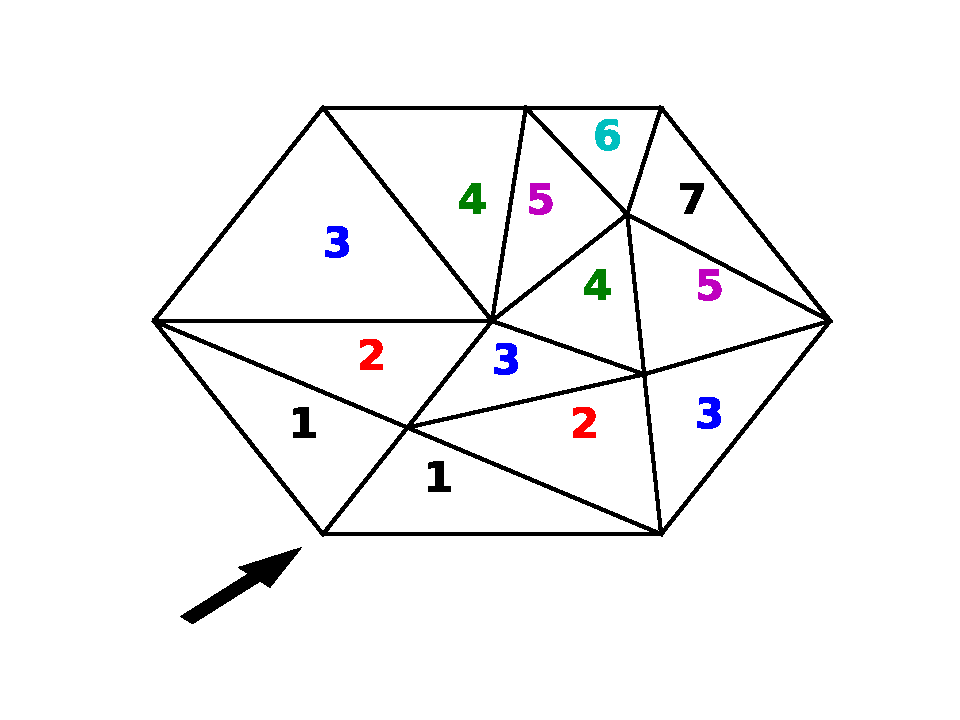
\includegraphics[scale=0.5]{../figures/UnstructuredMesh.pdf}
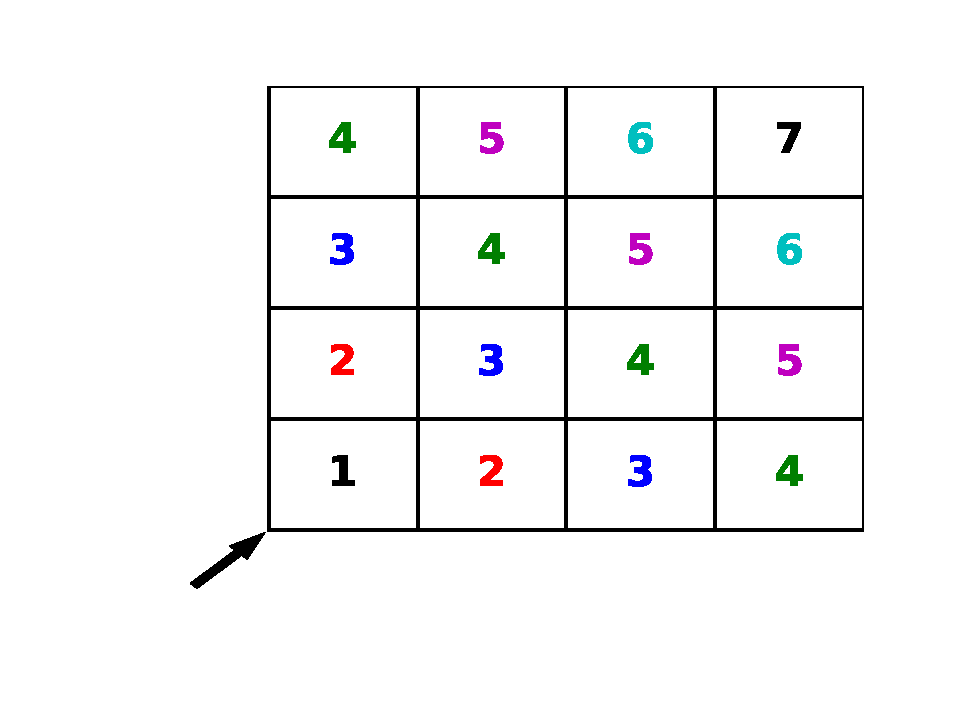
\includegraphics[scale = 0.5]{../figures/StructuredMesh.pdf}
\caption{A demonstration of a sweep on structured and unstructured meshes. }
\label{sweeps}
\end{figure}

The number in each cell represents the order in which the cells are solved.
Obtaining the solution for current cells in the sweep is dependent on the solution of downwind cells.
This process can be represented and stored as a task dependence graph, shown in Fig. \ref{tdg}.

\begin{figure}[H]
\centering
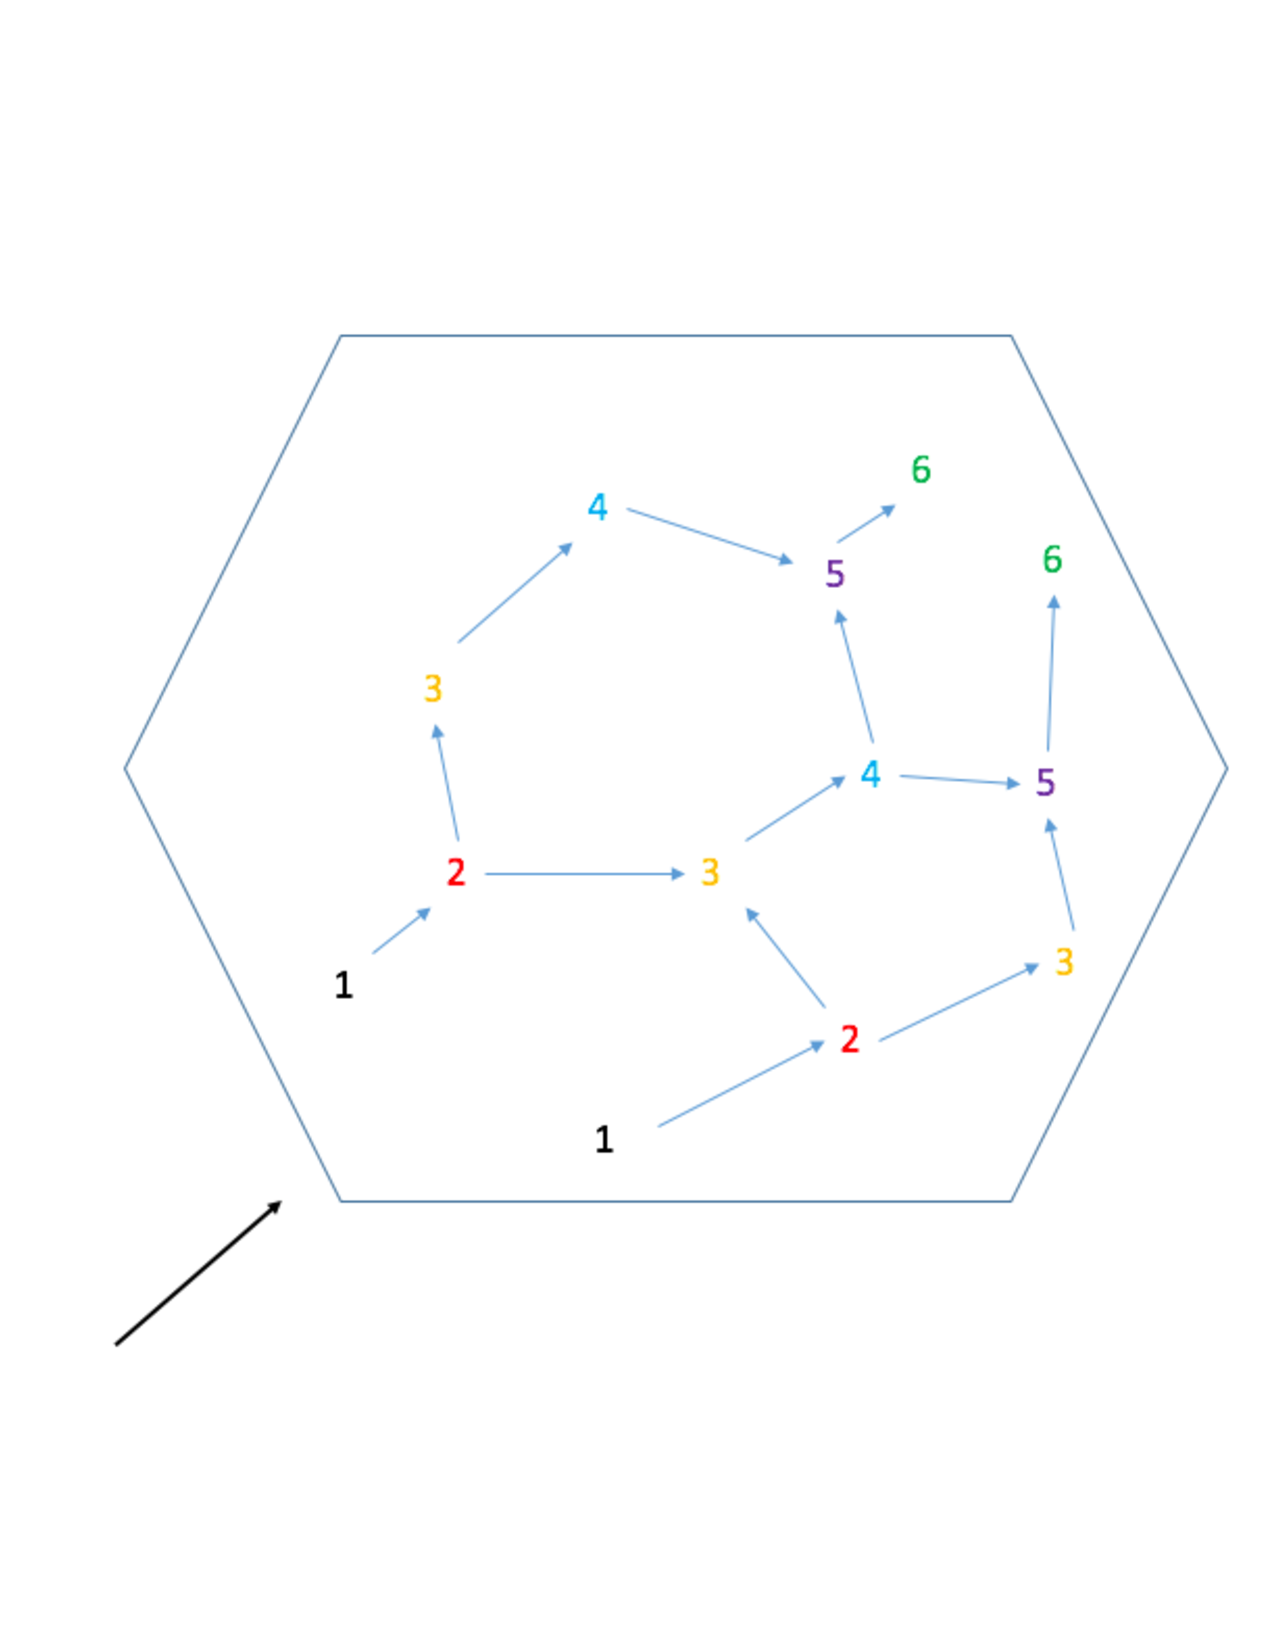
\includegraphics[scale = 0.35,trim={0cm 3cm 0cm 3cm},clip]{../figures/tdg.pdf}
\caption{A task dependence graph of the unstructured mesh example in Fig. \ref{sweeps}.}
\label{tdg}
\end{figure}

Massively parallel transport sweeps have been shown to scale up to 750,000 cores on logically Cartesian grids. However, structured meshes are somewhat limiting when  simulating more complex problems and experiments, requiring the use of unstructured meshes in transport sweeps. While unstructured meshes provide the ability to simulate realistic problems, they introduce some challenges like unbalanced partitions, which can increase the time to solution. To combat this, PDT, Texas A\&M University's massively parallel deterministic transport code, introduced two load balancing algorithms that rely on moving the spatial partition boundaries, or cut planes (cut lines in 2D), throughout the mesh in order to obtain a roughly equivalent amount of cells (and therefore work) per processor. However, this sacrifices the optimal partitioning scheme\cite{mpadams2013} in favor of balance. We propose a method that weighs ideal load balancing against the consequences to the transport sweep in order to achieve the best possible time to solution.



%%%%%%%%%%%%%%%%%%%%%%%%%%%%%%%%%%%%%%%%%%%%%%%%%%%
%
%  New template code for TAMU Theses and Dissertations starting Fall 2016.  
%
%
%  Author: Sean Zachary Roberson
%  Version 3.17.09
%  Last Updated: 9/21/2017
%
%%%%%%%%%%%%%%%%%%%%%%%%%%%%%%%%%%%%%%%%%%%%%%%%%%%

%%%%%%%%%%%%%%%%%%%%%%%%%%%%%%%%%%%%%%%%%%%%%%%%%%%%%%%%%%%%%%%%%%%%%%%
%%%                           SECTION II
%%%%%%%%%%%%%%%%%%%%%%%%%%%%%%%%%%%%%%%%%%%%%%%%%%%%%%%%%%%%%%%%%%%%%%


\chapter{PAGES WITH A FIGURE, A TABLE AND AN EQUATION}
\section{Figures: Placement, Size, and Captions}
This is a figure template.
\begin{figure}[ht]
\centering
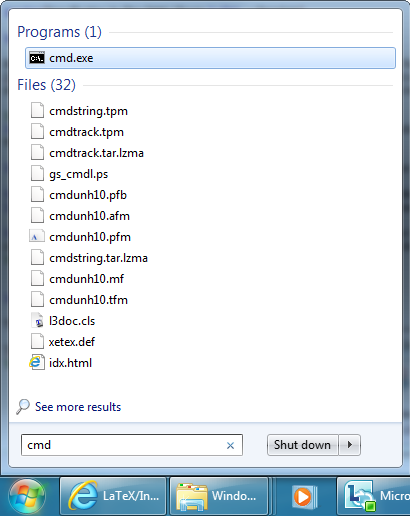
\includegraphics[scale=0.75]{TAMUthesis_CMD_windows.png}
\caption[The command line compiler in Windows.]{The command line compiler in Windows. It is not suggested that you compile using this method. See compilation instructions in the README.}

\label{fig:CMD_1}

\end{figure}

Figure (and table) titles should be consistent through the document. All captions should be placed either above or below the object it describes. This is done by placing the \textit{caption} in the correct place. While continued figures are allowed by the Thesis Manual, it is not suggested that any continued figures be included in a \LaTeX\ document. The figure below is from Linux Mint, showing a portion of a desktop.

\begin{figure}[H]
	\centering
	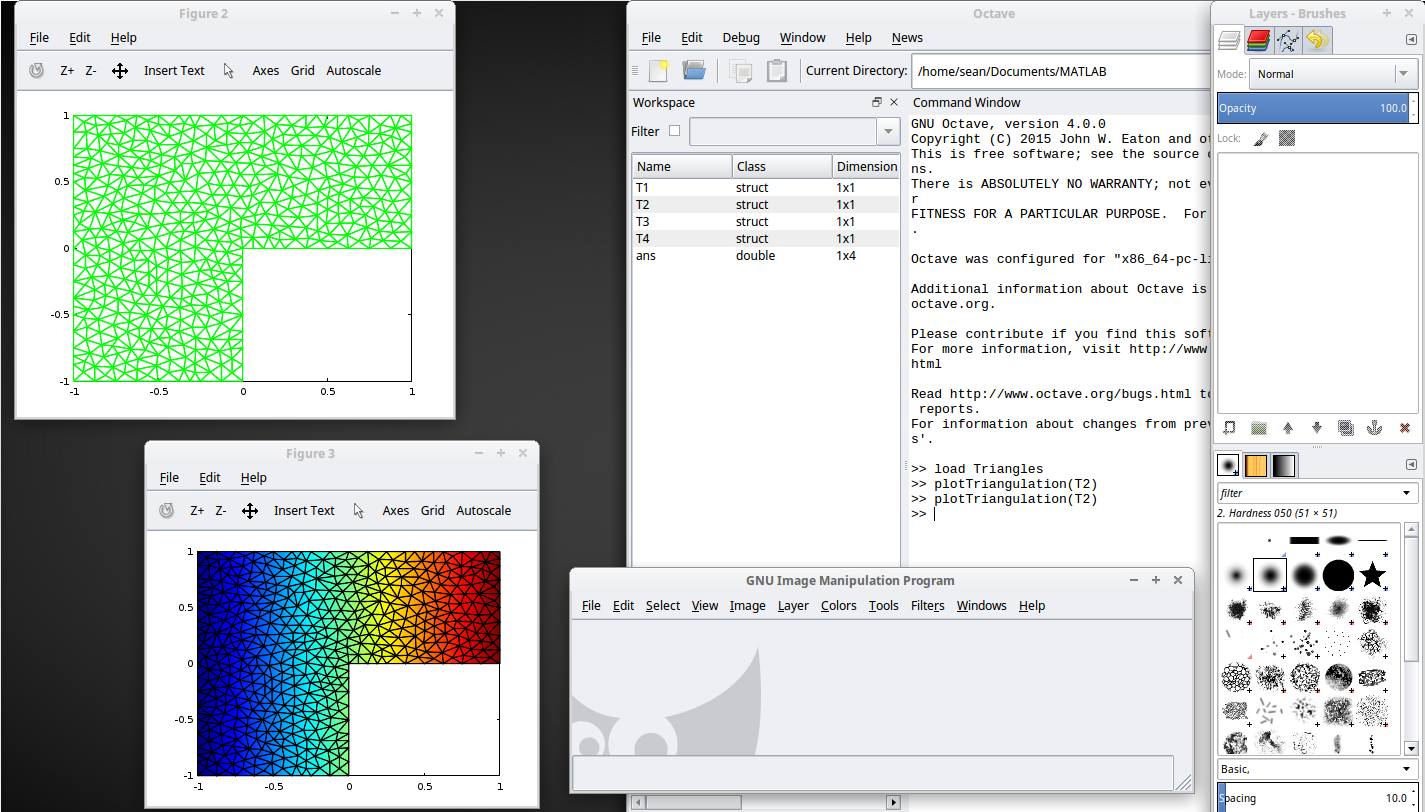
\includegraphics[width = 5.75in]{Desktop.png}
	\caption{A typical desktop space in Linux Mint.}
\end{figure}

The figure below is taken from R. While there are packages available to import graphics from R, MATLAB, and similar software, it is probably best to export plots generated by these programs as a PNG file, and then import it via the \textit{includegraphics} command.

\begin{figure}[H]
	\centering
	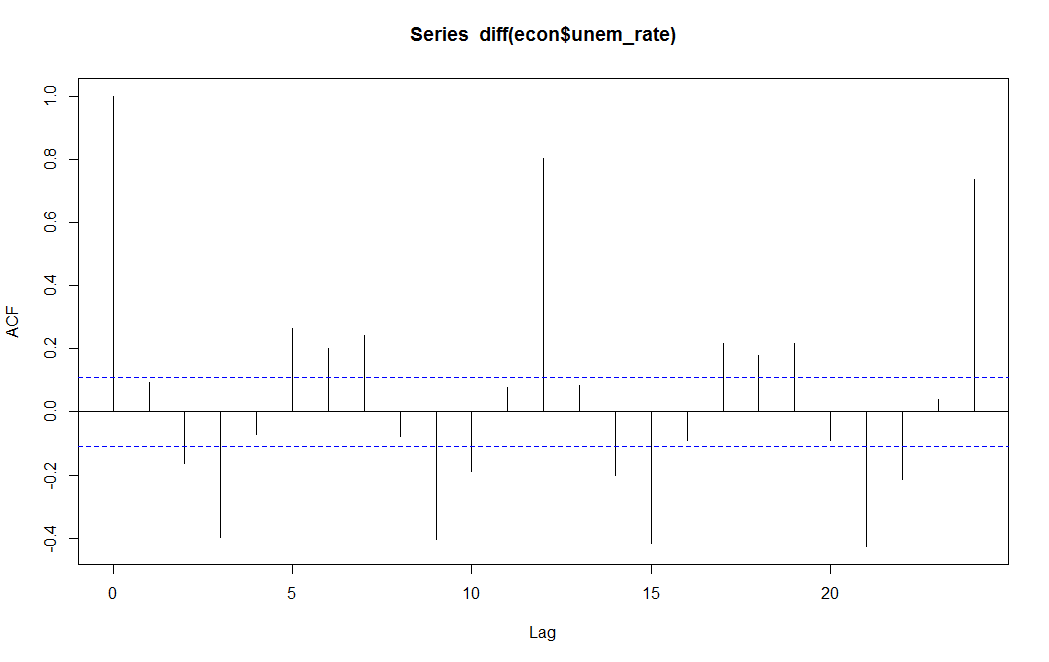
\includegraphics[scale=0.55]{UnemDiffACF.png}
	\singlespace
	\caption{The autocorrelation function (ACF) of the differenced unemployment series. Seasonal adjustments may be needed.}
\end{figure}

It is highly suggested that you scale the figures so that they fit within the margins. Almost all the figures included in this document for the sake of example have been scaled. It is best to use PNG and JPEG files as figures.

The last figure here is a screenshot from the Linux terminal.

\begin{figure}[H]
	\centering
	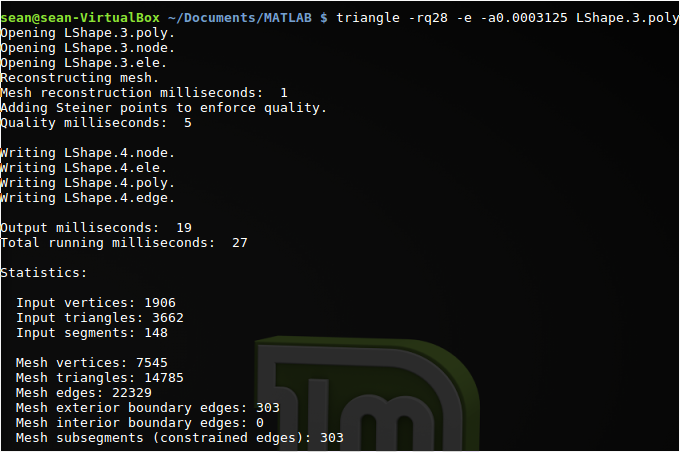
\includegraphics[width=4.75in]{Terminal1.png}
	\caption{The Linux terminal. The commands shown are from a two-dimensional mesh generator that triangulates a domain in the plane. Files containing nodes, elements, the polygon, and the edges are created.}
\end{figure}

\section{Table Placement, Size and Table Title}

Here is a table, displaying band and auxiliary scores from the 2011 Arcadia Festival of Bands held in Arcadia, CA \cite{ARCADIA}.

\begin{table}[h!]
	\centering

	\label{Band}
	\begin{tabular}{|l|l|l|}
		\hline
		School Name & Band Score & Auxiliary Score \\ \hline
		Rancho Bernardo & 96.15 & 89.15 \\ \hline
		Mt. Carmel & 95.30 & 83.55 \\ \hline
		Riverside King & 93.85 & 91.75 \\ \hline
		Diamond Bar & 93.20 & 88.60 \\ \hline
		El Dorado & 92.80 & 95.45 \\ \hline
		Chino & 92.65 & 91.45 \\ \hline
		Henry J. Kaiser & 92.60 & 87.55 \\ \hline
		Glendora & 92.60 & 89.15 \\ \hline
		Montebello & 90.50 & 82.70 \\ \hline
		Mira Mesa & 89.65 & 91.50 \\ \hline
	\end{tabular}
	\caption{Scores from the 2011 Arcadia Festival of Bands.}
\end{table}

The table is sorted by band score. There is more text here to demonstrate how the template handles spacing between tables and body text. Also note how the table caption is in a smaller font size than the body text.

\section{Equations}

The following format is recommended to be used to display equations.

%Make other examples.
\begin{equation} \label{Equ.2.1}
y=c_1\cos(t)+c_2\sin(t)
\end{equation}
\begin{equation} \label{Equ.2.2}
e^{it}=\cos(t)+i\sin(t)
\end{equation}

Equation \ref{Equ.2.1} is the general solution to the differential equation $y''+y=0$. In the source code, the \textit{ref} command allows you to refer to an equation by a label you created. References must be made after the equation has been created; attempting to refer to an equation before it is defined results in a question mark placeholder. Some more sample equations are below. Notice the first set below is not numbered.
%%
\begin{align*}
\log (x^n) &= \log (x \cdot x \cdot \ldots \cdot x) \\
&= \log x + \log x + \ldots + \log x \\
&= n \log x
\end{align*}
\begin{equation} \label{Equ.2.3}
X^T X \mathbf{u} = X^T \mathbf{y}
\end{equation}
\begin{equation}\label{Equ.2.4}
u(x, t) = \int_{-\infty}^{\infty} G(x, \tau) \exp\left(-\frac{(t-\tau)^2}{4kt}\right) \ d\tau
\end{equation}
\begin{gather}
\mathcal{L}(f) = \int_{0}^{\infty} e^{-st} f(t) \ dt \\
\begin{split} \label{Equ.2.5}
\mathcal{F}(f) = \frac{1}{2\pi}\int_{-\infty}^{\infty} e^{i \omega x} f(x) \ dx
\end{split}
\end{gather}

You can use labels to refer to equations you create. \ref{Equ.2.5} is the \textbf{Laplace transform} used extensively in differential equations. \ref{Equ.2.3} is the matrix representation of the \textbf{normal equations} used in least-squares regression.

To have equations without labels appearing the right margin, simply add an asterisk to the name of the environment (equation, align, etc.) when making the declaration.


\section{Theorems and Proofs: Examples}

This section will show an example usage of the theorem and proof environments, typically used for mathematics students. To use these environments, you must have the package \textbf{amsthm} declared in the preamble of your document. For this template, this is already declared in the main file. You may choose to remove this declaration if your document will not make use of theorems and proofs.

Theorems can be numbered, as the one below is, or you can force a different label to appear. For example, you can state the Bolzano-Weierstass theorem and have the names appear as the theorem label. See the examples below.

Sometimes you may have a theorem with multiple parts or multiple conditions. You can use other list environments, such as enumerate, inside the theorem environment declared to list these conditions. The final example at the end of this block shows this with the Invertible Matrix Theorem, which has several equivalent statements.

\newtheorem{thm}{Theorem}
\begin{thm}
	Suppose $f$ is of class $\mathcal{C}^1$ and $g$ is of class $\mathcal{C}^2$, and that the compact set $D$ and its boundary satisfy the hypotheses of Green's Theorem.  Then
	\[ \iint \limits_D f\nabla^2 g \ dA = \oint_{\partial D} f(\nabla g) \cdot \mathbf{n} \ ds - \iint \limits_D \nabla f \cdot \nabla g \ dA . \]
\end{thm}

\begin{proof}
	Begin with the integral of $f\nabla g \cdot n$ taken over the boundary of D.  By the second vector form of Green's Theorem,
	\begin{align*}
	\oint_{\partial D} f\nabla g \cdot n \ ds &= \iint \limits_D \nabla \cdot (f\nabla g) \ dA \\
	&= \iint \limits_D f\nabla^2 g + \nabla f \cdot \nabla g \ dA.
	\end{align*}
	
	Rearranging yields the desired.
\end{proof}

\begin{thm}[Bolzano-Weierstrass]
	Every bounded real sequence has a convergent subsequence.
\end{thm}

\begin{thm}[Invertible Matrix Theorem\footnote{This is an incomplete list.}]
	For any square matrix $A$ with $n$ rows and columns, the following are equivalent.
	\begin{enumerate}
		\item $A$ is invertible.
		\item The equation $A\mathbf{x}=\mathbf{0}$ has only the trivial solution $\mathbf{x} = \mathbf{0}.$
		\item For any nonzero $\mathbf{b}, \ A\mathbf{x} = \mathbf{b}$ has exactly one solution.
		\item The columns of $A$ form a linearly independent set.
		\item Zero is not an eigenvalue of $A$.
		\item $A$ has full rank.
		\item The determinant of $A$ is not zero.
	\end{enumerate}
\end{thm}

There is currently no set format on how propositions and theorems should be laid out in the document. The idea is to remain consistent. It is best to not customize the appearance of theorems so that they can easily be distinguished from body text - just like figures, tables, and headings.

\section{Another Table Example}
For the sake of testing the appearance of the list of tables, a second table will be displayed here. This table displays a list of some major universities and their enrollments during fall 2015. This table is sorted in descending order of enrollment.
%The savenotes environment, loaded from the footnote package
%(which in turn is loaded from mdwtools)
%allows you to use footnotes in tables, if needed.
\begin{savenotes}
\begin{table}[h!]
	\centering
	\label{my-label}
	\begin{tabular}{|l|l|l|}
		\hline
		School & City and State & Fall 2015 Enrollment  \\ \hline
		Texas A\&M University\footnote{Gig 'em!} & College Station, TX & 64,376  \\ \hline
		Ohio State University\footnote{This number describes enrollments at the Columbus campus; enrollments at regional campuses in Lima, Mansfield, Marion, Newark, and Wooster are not counted.} & Columbus, OH & 58,322 \\ \hline
		Iowa State University & Ames, IA & 36,001 \\ \hline
		University of California, San Diego & La Jolla, CA & 33,735   \\ \hline
		University of West Florida & Pensacola, FL & 12,798 \\ \hline
		Massachusetts Institute of Technology & Cambridge, MA & 11,319   \\ \hline
	\end{tabular}
	\caption{Some major universities and their fall 2015 enrollments.}
\end{table}
\end{savenotes}

Naturally, tables and footnotes do not go together. If you attempted to write a footnote inside a table, there will be nothing at the bottom of the page, yet the footnote marker will still appear. To remedy this, the \textit{footnote} package has been loaded from the \textit{mdwtools} package. Check your TeX distribution to see if \textit{mdwtools} is installed. See the source code for how this is implemented.

Here are some blank floats.

\begin{figure}[!h]
	\caption{A blank float.}
\end{figure}

\begin{figure}[!h]
	\caption{Another blank float.}
\end{figure}
%%%%%%%%%%%%%%%%%%%%%%%%%%%%%%%%%%%%%%%%%%%%%%%%%%%
%
%  New template code for TAMU Theses and Dissertations starting Fall 2016.  
%
%
%  Author: Sean Zachary Roberson
%  Version 3.17.09
%  Last Updated: 9/21/2017
%
%%%%%%%%%%%%%%%%%%%%%%%%%%%%%%%%%%%%%%%%%%%%%%%%%%%
%%%%%%%%%%%%%%%%%%%%%%%%%%%%%%%%%%%%%%%%%%%%%%%%%%%%%%%%%%%%%%%%%%%%%%
%%                           SECTION III
%%%%%%%%%%%%%%%%%%%%%%%%%%%%%%%%%%%%%%%%%%%%%%%%%%%%%%%%%%%%%%%%%%%%%

\chapter{LOAD BALANCING UNSTRUCTURED MESHES}

Initially, PDT only swept on structured, logically Cartesian meshes. As the need to solve problems with more complex geometries arose, PDT added a support for arbitrary polyhedral unstructured meshes. However, this introduced imbalanced partitions, causing longer and unmanageable runtimes.

To combat imbalanced partitions, two load balancing algorithms were implemented, referred to in this paper as the original load balancing algorithm and the load balancing by dimension algorithm.

Before detailing the two load balancing algorithms PDT employs, a quick review of partitioning unstructured meshes in PDT is necessary:
%\vspace{-2.5cm}
\begin{itemize}\itemsep 1pt \parskip 0pt \parsep 0pt
\item ``Cut lines" in 2D (cut planes for 3D) are used to slice through the mesh in the $x$, $y$, and $z$ dimensions.
\item The cut planes form brick partitions, called subsets, that have unstructured meshes inside of them. 
\item The subsets are distributed amongst the processor domain.
\end{itemize}
%\vspace{-2cm}
Figure \ref{partitioning_example} shows an example of an unstructured mesh partitioned into four subsets in PDT. 

\begin{figure}[H]
\centering
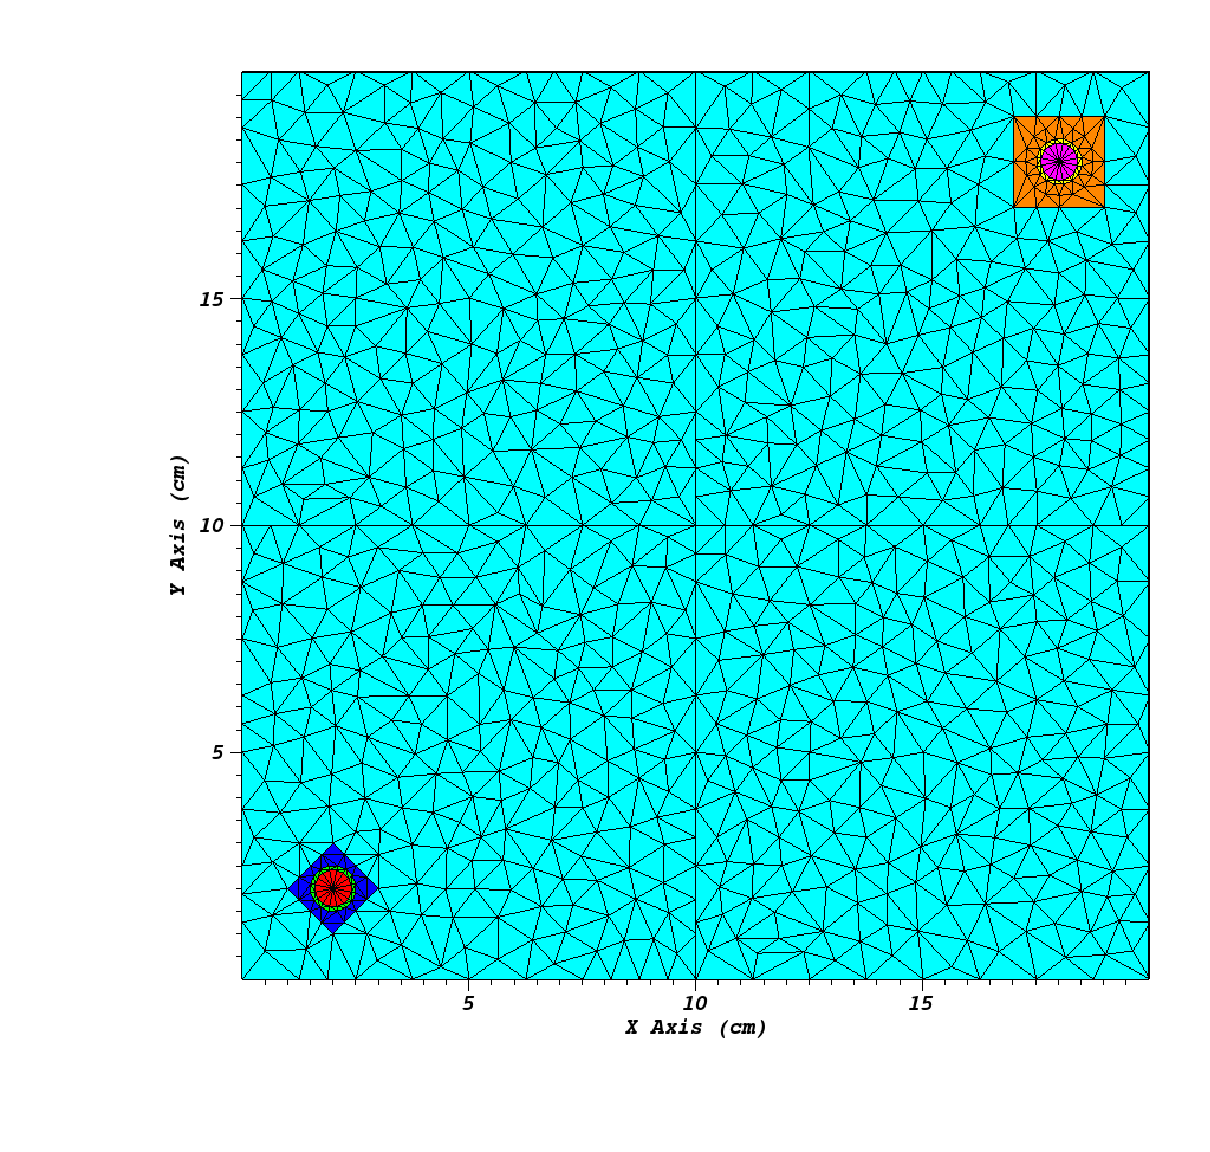
\includegraphics[scale=0.4,trim={0.95in 0.64in 0.35in 0.44in},clip]{Figures/partitioning_example.pdf}
\caption{An unstructured mesh partitioned into four subsets with cut planes at $\bm{x,y = 10}$ cm.}
\label{partitioning_example}
\end{figure}
Both approaches to load balancing move these cut planes in order to redistribute cells more evenly throughout subsets. We define a metric describing how imbalanced our problem is:
\begin{equation}
f =\frac{\underset{ijk}{\text{max}}(N_{ijk})}{\frac{N_{tot}}{I\cdot J\cdot K}},
\label{metric_def}
\end{equation}
where $f$ is the load balance metric, $N_{ijk}$ is the number of cells in subset $(i,j,k)$, $N_{tot}$ is the global number of cells in the problem, and $I$, $J$, and $K$ are the total number of subsets in the $x$, $y$, and $z$ direction, respectively. The metric is a measure of the maximum number of cells per subset divided by the average number of cells per subset. For a perfectly balanced problem, $f = 1$.

Dimensional sub-metrics are defined to assist with the movement of the partitions:
\begin{equation}
f_{D} = \underset{d}{\text{max}}[\sum_{d2,d3} N_{ijk}]/\frac{N_{tot}}{D}.
\label{f_d}
\end{equation}
$f_{D}$ is calculated by taking the maximum number of cells per row, column, or plane and dividing it by the average number of cells per the corresponding dimension. If this number is greater than predefined tolerances, the cut planes in the respective dimension are redistributed. 

Figure \ref{redistribute} illustrates an example of redistributing the cut planes in $x$ to balance the cells per column.
\begin{figure}[H]
\centering
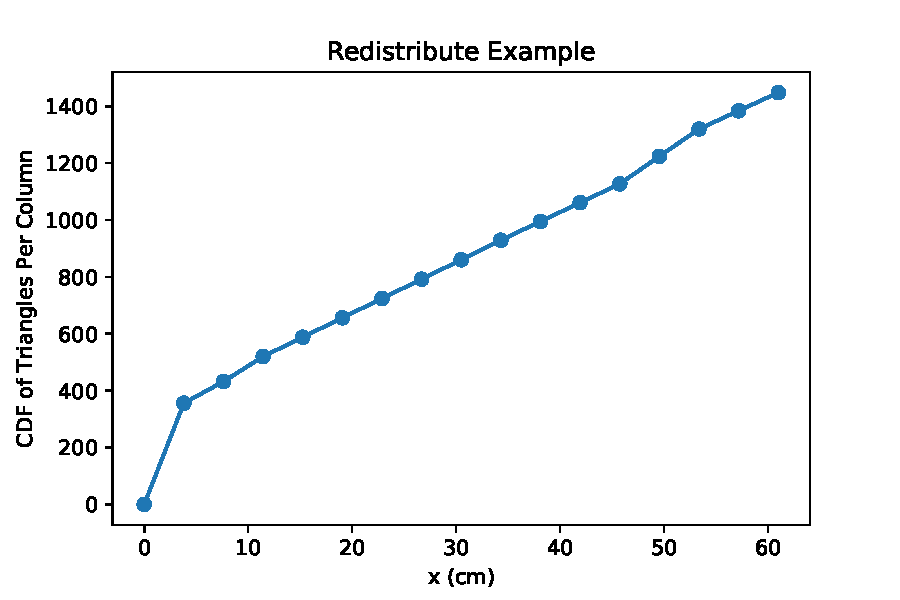
\includegraphics[scale=0.4]{Figures/redistribute_before.pdf}
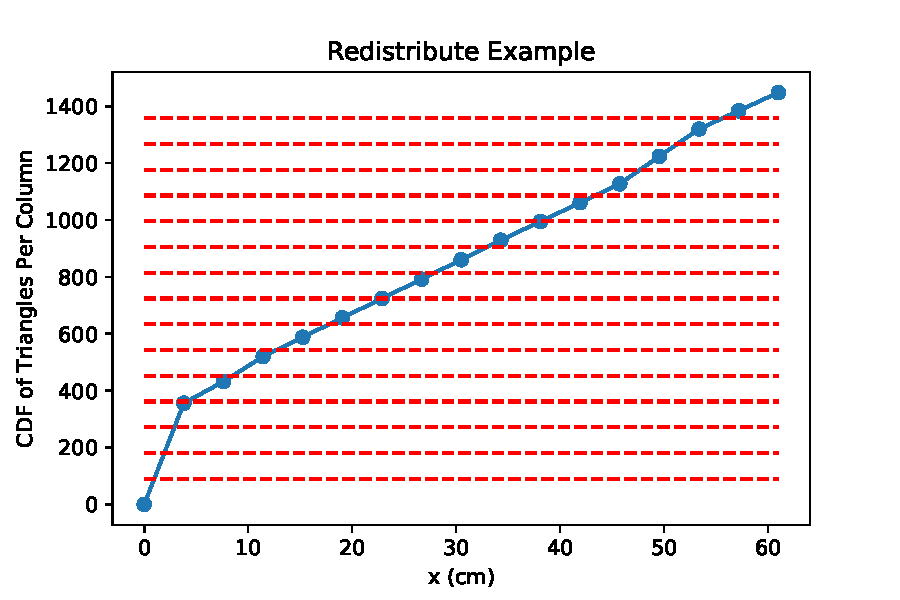
\includegraphics[scale=0.4]{Figures/redistribute_after.pdf}
\caption{The use of the CDF of triangles per column to redistribute the cut planes in X.}
\label{redistribute}
\end{figure}
The image on the left side of Fig. \ref{redistribute} shows the CDF of the triangles per column. The red lines on the right side of Fig. \ref{redistribute} show the ideal equal number of cells per column. The x-value of the intersection of these red lines and the CDF are where the cut planes are redistributed to. 
 
\section{Original Load Balancing Algorithm}

The initial approach to load balancing was implemented on 2D extruded meshes, meaning the mesh is balanced in the 2D plane and then extruded, yielding a balanced 3D mesh. Algorithm \ref{initial_algorithm} summarizes the initial approach to load balancing meshes in PDT.

\begin{algorithm}[H]
\caption{The original load balancing algorithm.}
\label{initial_algorithm}
\begin{algorithmic}

\WHILE{$f > \text{tol}_{\text{subset}}$}
  \IF {$f_I > \text{tol}_{\text{col}}$}
    \STATE Redistribute the X cut planes.
  \ENDIF
  \IF {$f_J > \text{tol}_{\text{row}}$}
  	\STATE Redistribute the Y cut planes.
  \ENDIF
\ENDWHILE
\end{algorithmic}
\end{algorithm}
While the problem is not balanced, we check if the cells per column and cells per row, represented by $f_I$ and $f_J$ (defined by Eq. (\ref{f_d})), are balanced. If they are not, we redistribute the corresponding cut planes.
%\vspace{-3.5cm}

The original load balancing algorithm placed cut planes in all dimensions all the way through the mesh. This created an orthogonal partitioning where each subset had an equivalent number of neighbors, which was done to preserve the optimal sweep partitioning described by Adams et. al \cite{mpadams2015}. However, there are theoretical limits to load balancing in this fashion. Figure \ref{2dgeneral} shows a simple 2D subset layout with $M$ unaligned patches of high mesh density.

\begin{figure}[H]
\centering
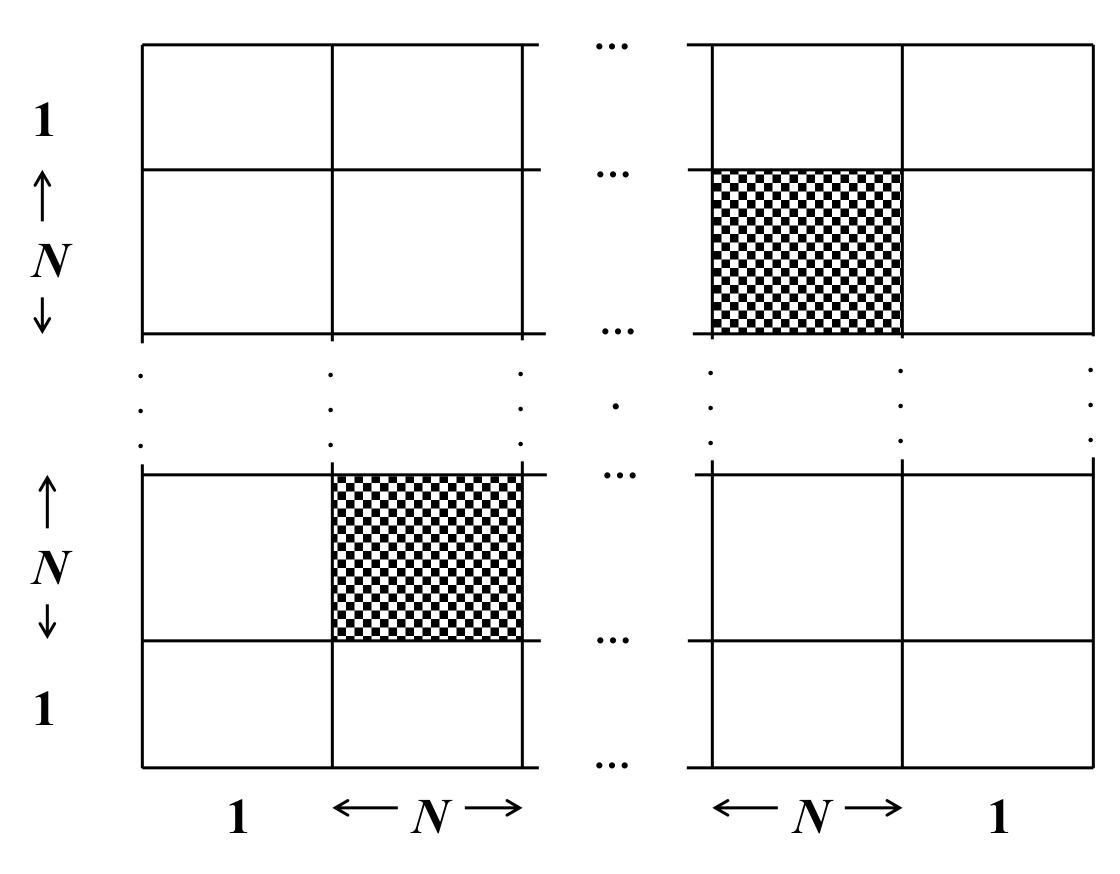
\includegraphics[scale=0.4]{Figures/2dgeneral.png}
\caption{A 2D subset layout with $M$ unaligned patches of high mesh density.}
\label{2dgeneral}
\end{figure}

The subset layout is $[M(N+1)+1] \times [M(N+1)+1]$, but only $MN^2$ subset have significant work, leading to a theoretical limit for the load imbalance factor:
\begin{equation}
f= \frac{\left( M(N+1)+1 \right)^2}{MN^2} \xrightarrow{N\to \infty} \frac{M^2N^2}{MN^2} = M.
\end{equation}

Due to this theoretical limit, the load balancing by dimension algorithm was developed.

\section{Load Balancing by Dimension Algorithm}

The load balancing by dimension algorithm, like the original load balancing algorithm, relies on the movement of cut planes to redistribute mesh cells in a more balanced manner. However rather than moving all cut planes in all dimensions in one iteration, one dimension is balanced first for all iterations, and then the cut planes that yield the best metric for that dimension are chosen. Then the next dimensions is balanced within the first dimension. For example, if the $x$ cut planes are balanced first, the $y$ cut planes are balanced \textit{within} each column.
We slightly alter the definition for our dimensional sub-metrics (Eq. (\ref{f_d})) accordingly:
\begin{align}
f_{D1} &= \underset{d1}{\text{max}}[\sum_{d2,d3} N_{ijk}]/\frac{N_{tot}}{D1}, \label{f_d1} \\
f_{D2,d1} &= \Big(\underset{d2}{\text{max}}[\sum_{d3} N_{ijk,d1}]/\frac{N_{d1}}{D2}\Big), \label{f_d2}\\
f_{D3,d2,d1} &= \Big( \underset{d3}{\text{max}}[ N_{ijk,d1,d2}]/\frac{N_{d1,d2}}{D3} \Big) . \label{f_d3}
\end{align}
Equation (\ref{f_d1}) represents the sub-metric for the first dimension we load balance. In order to assist in the explanation of $f_{D2,d1}$ and $f_{D3,d2,d1}$, we'll take $D1$ to be the $z$ dimension. In Eq. ({\ref{f_d1}), $D1$ represents the number of $z$ planes, $N_{tot}$ represents the number of cells in the mesh, and $N_{ijk}$ is the number of cells in subset $(i,j,k)$. $f_{D1}$ is the maximum number of cells per plane by the average number of cells per plane. 

Once the z planes are balanced according to $f_{D1}$, we balance the second dimension (in this example, the columns, or $x$ cut planes) \textit{within} each $z$ plane. $f_{D2,d1}$ represents the column-wise sub-metrics for each $z$ plane. In other words, there are $D1$ column-wise sub-metrics, one for each plane. These column-wise sub-metrics are calculated by dividing the maximum number of cells per column divided by the average number cells per column \textit{in each plane}. 

Once the columns within each z-plane are balanced, we balance the rows $within$ the columns $within$ each plane. The row-wise sub-metrics for each plane for each column, $f_{D3,d2,d1}$, are calculated by dividing the maximum number of cells per row per column by the average number of cells per row per column in each plane. Algorithm \ref{lbd} summarizes the load balancing by dimension process described. 

\begin{algorithm}[H]
\caption{The load balancing by dimension algorithm.}
\label{lbd}
\begin{algorithmic}

  \WHILE {$f_{D1} > \text{tol}_{\text{D1}}$}
    \STATE Redistribute the D1 cut planes.
  \ENDWHILE  
  
  \FOR {$d1$ in $D1$}
    \WHILE {$f_{D2,d1} > \text{tol}_{\text{D2}}$}
      \STATE Redistribute the D2 cut planes within d1. 
    \ENDWHILE
  \ENDFOR
  
  \FOR{$d1$ in $D1$}
    \FOR{$d2$ in $D2$}
      \WHILE {$f_{D3,d2,d1} > \text{tol}_{\text{D3}}$ }
        \STATE Redistribute the D3 cut planes within d2 within d1. 
      \ENDWHILE
    \ENDFOR
  \ENDFOR
  
  \STATE Calculate $f$.
\end{algorithmic}
\end{algorithm}

Figure \ref{alg_illustration} illustrates the behavior of both algorithms. In the left image of the figure, we see the partitions cutting across the entire domain, with the left-most $x$ cut line moved into the denser geometric feature in the bottom left corner to more evenly distribute cells. In the right image of the figure, we see the $x$ partitions cutting across the entire domain, but the $y$ partitions being redistributed by column. The $y$ partitions are moved into the respective geometric features in the appropriate columns in order to better balance the problem.

\begin{figure}[H]
\centering
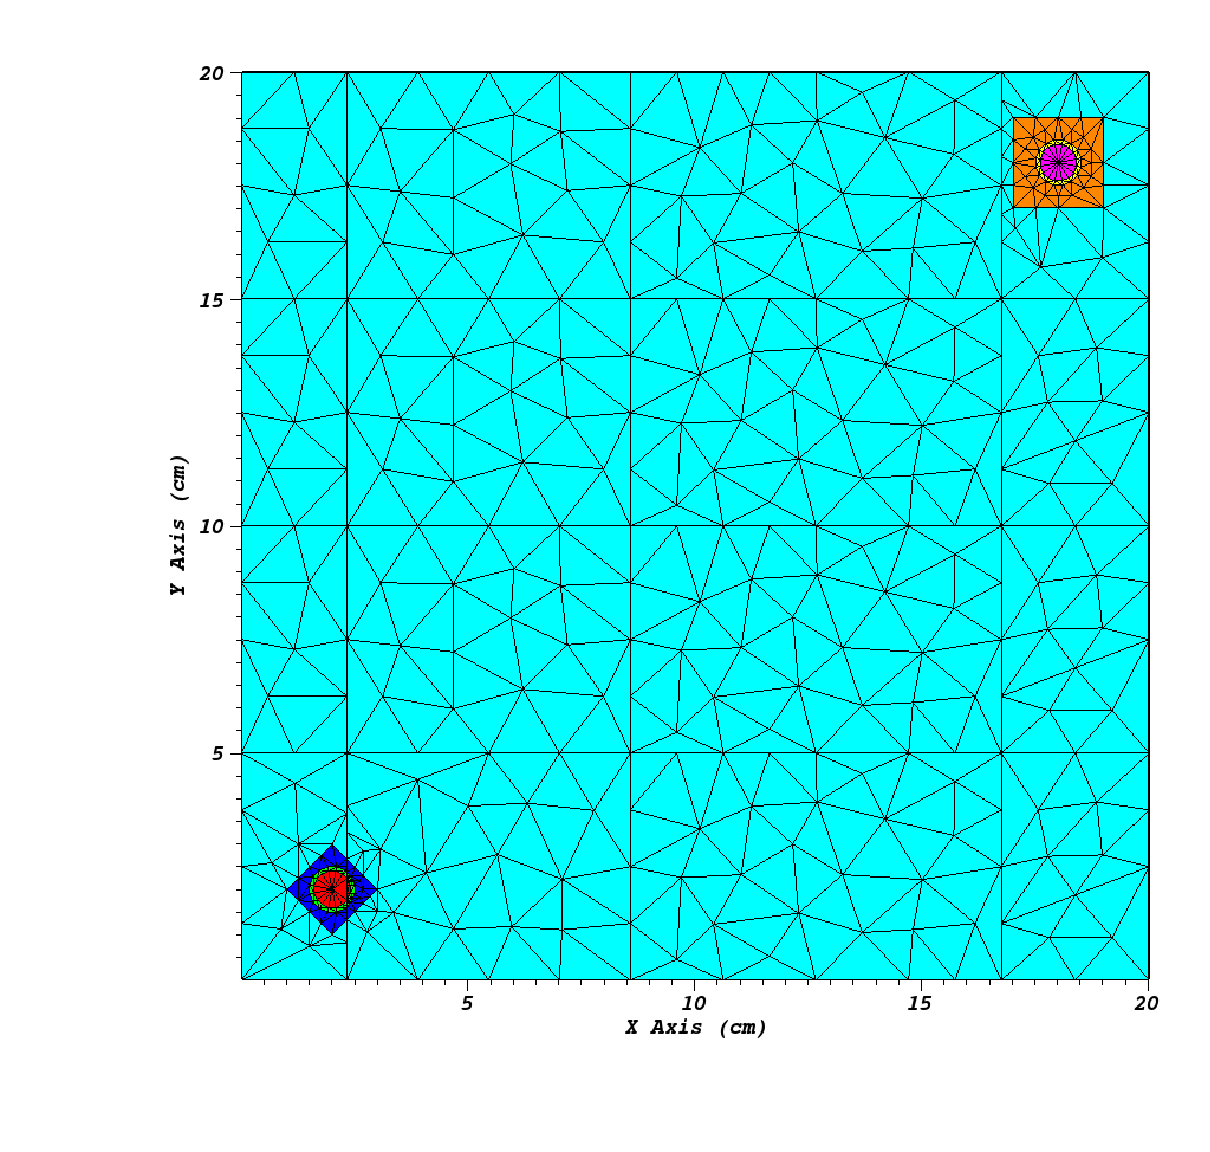
\includegraphics[scale=0.45,trim={0.95in 0.64in 0.35in 0.44in},clip]{Figures/og_lb_example.pdf}
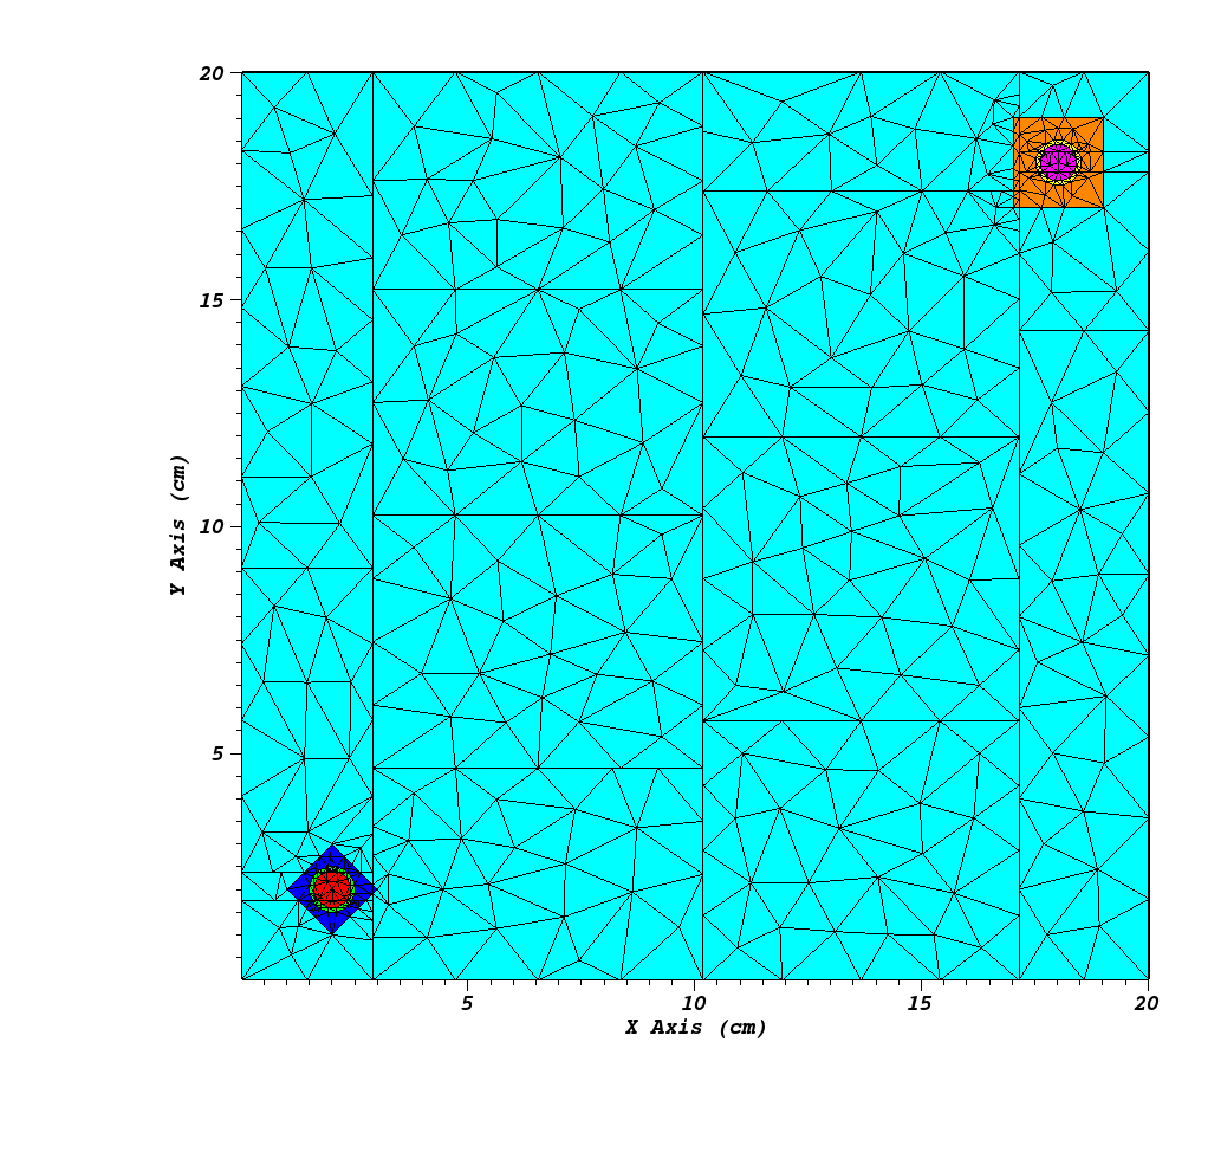
\includegraphics[scale=0.45,trim={0.95in 0.64in 0.35in 0.44in},clip]{Figures/lbd_example.pdf}
\caption{The partitions of a problem after the original load balancing (left) and the load balancing by dimension (right) algorithms.}
\label{alg_illustration}
\end{figure}


\section{RESULTS}

To show the behavior of the original load balancing algorithm and the load balancing by dimension algorithm, the problem shown in Fig. \ref{partitioning_example} was run with a varying number of subsets and with a varying maximum triangle area, with the minimum allowable angle per triangle was kept constant at \ang{20}. We varied the number of subsets in $x$ and $y$ from 2 to 10 (with the total number of subsets varying from 4 to 100). The problem illustrated by Fig. \ref{partitioning_example} was chosen because it has two dense features in opposing corners with no features in between, lending itself to being an imbalanced mesh. Table \ref{og_table} shows the results of this parametric study using the original load balancing algorithm vs. using the load balancing by dimension algorithm. Table \ref{all_improvements} shows the percent improvements for both algorithms from no load balancing to running both load balancing algorithm, while Table \ref{method_improvement} shows the improvement of the load balancing by dimension algorithm relative to the original load balancing algorithm.

%\vspace{-1cm}
\begin{table}[H]
\centering
  \caption{\bf The results of the parametric study using the original load balancing algorithm (left) and the load balancing by dimension algorithm (right).}
  \scalebox{0.5}{
  \begin{tabular}{c|c|c|c|c|c|c|c|c|c} 
  \bf Area, $N^{1/2}$ & \bf  2 &  \bf 3    &  \bf  4   &  \bf  5   &  \bf  6   &  \bf  7   & \bf   8   &  \bf 9    &  \bf 10   \\ \hline \hline
\bf Coarse&1.993 & 2.735 & 4.360 & 4.812 & 5.545 & 6.321 & 3.114 & 2.697 & 1.893 \\ \hline 
\bf 1.8& 1.408 & 2.277 & 2.886 & 3.269 & 4.716 & 4.721 & 5.890 & 4.618 & 1.863 \\ \hline
\bf 1.6& 1.375 & 2.206 & 2.649 & 3.247 & 4.356 & 4.876 & 4.678 & 5.062 & 1.329 \\ \hline
\bf 1.4& 1.337 & 2.110 & 2.982 & 3.031 & 4.615 & 4.310 & 8.911 & 4.652 & 2.675 \\ \hline
\bf 1.2& 1.344 & 2.008 & 2.017 & 3.392 & 3.916 & 4.969 & \cellcolor{blue!25}9.576 & 4.543 & 4.728 \\ \hline
\bf 1.0& 1.264 & 1.806 & 2.405 & 2.976 & 3.657 & 4.317 & 6.242 & 4.831 & 4.941 \\ \hline
\bf 0.8& 1.212 & 1.640 & 2.300 & 2.436 & 2.941 & 4.395 & 7.420 & 4.466 & 3.947 \\ \hline
\bf 0.6& 1.153 & 1.567 & 2.045 & 2.368 & 3.199 & 2.999 & 7.206 & 4.101 & 3.592 \\ \hline
\bf 0.4& 1.108 & 1.411 & 1.633 & 2.117 & 2.383 & 2.646 & 6.970 & 3.086 & 2.511 \\ \hline
\bf 0.2& 1.052 & 1.197 & 1.258 & 1.523 & 1.789 & 1.857 & 3.380 & 2.193 & 1.883 \\ \hline
\bf 0.1& 1.029 & 1.092 & 1.149 & 1.207 & 1.276 & 1.420 & 2.015 & 1.565 & 1.247 \\ \hline
\bf 0.08& 1.009 & 1.043 & 1.086 & 1.101 & 1.179 & 1.267 & 2.118 & 1.551 & 1.271 \\ \hline
\bf 0.06& 1.009 & 1.024 & 1.059 & 1.094 & 1.138 & 1.154 & 1.825 & 1.432 & 1.138 \\ \hline
\bf 0.05& 1.008 & 1.023 & 1.025 & 1.028 & 1.073 & 1.149 & 1.666 & 1.380 & 1.110 \\ \hline
\bf 0.04& 1.005 & 1.016 & 1.017 & 1.021 & 1.038 & 1.051 & 1.520 & 1.311 & 1.080 \\ \hline
\bf 0.03& 1.005 & 1.008 & 1.018 & 1.039 & 1.059 & 1.073 & 1.450 & 1.179 & \cellcolor{red!25}1.001 \\ \hline
\bf 0.02& 1.005 & 1.008 & 1.010 & 1.013 & 1.021 & 1.035 & 1.623 & 1.137 & 1.016 \\ \hline
\bf 0.01& 1.003 & 1.009 & 1.009 & 1.011 & 1.016 & 1.013 & 1.281 & 1.058 & 1.015 \\ \hline
  \end{tabular}}
 \scalebox {0.5}{
   \begin{tabular}{c|c|c|c|c|c|c|c|c|c} 
\bf Area, $N^{1/2}$ & \bf  2 & \bf 3    &  \bf  4   &  \bf  5   &  \bf 6    &  \bf  7   &   \bf 8   &  \bf 9    &  \bf 10   \\ \hline \hline
\bf Coarse & 1.645 & 1.455 & 1.878 & 2.348 & 3.046 & 3.022 & 1.752 & 2.304 & 1.451 \\ \hline 
\bf 1.8& 1.034 & 1.460 & 2.127 & 1.744 & 2.098 & 2.588 & 2.623 & 2.776 & 2.872 \\ \hline
\bf 1.6& 1.015 & 1.396 & 1.899 & 1.877 & 2.090 & 2.857 & 2.608 & 3.582 & 2.604 \\ \hline
\bf 1.4& 1.011 & 1.418 & 1.631 & 1.964 & 1.820 & 2.968 & 2.055 & 2.201 & 1.523 \\ \hline
\bf 1.2& 1.019 & 1.344 & 1.483 & 1.983 & 2.122 & 3.023 & 2.356 & \cellcolor{blue!25}4.765 & 2.371 \\ \hline
\bf 1.0& 1.007 & 1.338 & 1.641 & 2.313 & 3.097 & 2.098 & 2.563 & 2.808 & 2.637 \\ \hline
\bf 0.8& 1.016 & 1.157 & 1.457 & 1.982 & 1.881 & 2.340 & 2.283 & 3.513 & 3.947 \\ \hline
\bf 0.6& 1.012 & 1.111 & 1.199 & 1.598 & 1.901 & 1.791 & 2.330 & 3.005 & 3.719 \\ \hline
\bf 0.4& 1.005 & 1.024 & 1.204 & 1.288 & 1.665 & 1.492 & 1.660 & 2.528 & 2.511 \\ \hline
\bf 0.2& 1.007 & 1.021 & 1.025 & 1.116 & 1.175 & 1.358 & 1.478 & 1.624 & 1.837 \\ \hline
\bf 0.1& 1.003 & 1.019 & 1.024 & 1.019 & 1.092 & 1.122 & 1.161 & 1.087 & 1.247 \\ \hline
\bf 0.08& 1.007 & 1.010 & 1.022 & 1.035 & 1.035 & 1.077 & 1.176 & 1.135 & 1.219 \\ \hline
\bf 0.06& 1.004 & 1.009 & 1.021 & 1.032 & 1.031 & 1.070 & 1.102 & 1.080 & 1.072 \\ \hline
\bf 0.05& 1.002 & 1.005 & 1.019 & 1.023 & 1.038 & 1.071 & 1.096 & 1.094 & 1.101 \\ \hline
\bf 0.04& 1.002 & 1.008 & 1.008 & 1.021 & 1.027 & 1.028 & 1.063 & 1.091 & 1.080 \\ \hline
\bf 0.03& 1.003 & 1.008 & 1.013 & 1.014 & 1.030 & 1.044 & 1.068 & 1.074 & \cellcolor{red!25}1.001 \\ \hline
\bf 0.02& 1.002 & 1.006 & 1.009 & 1.013 & 1.020 & 1.030 & 1.038 & 1.058 & 1.016 \\ \hline
\bf 0.01& \cellcolor{red!25}1.001 & 1.006 & 1.007 & 1.011 & 1.015 & 1.013 & 1.030 & 1.029 & 1.015 \\ \hline

  \end{tabular}} 
  \label{og_table}
\end{table}

\begin{table}[H]
\centering
\caption{\bf The percent improvement of the original load balancing algorithm (left) and the load balancing by dimension algorithm (right).}
\scalebox{0.5}{
\begin{tabular}{c|c|c|c|c|c|c|c|c|c} 

\bf Area, $N^{1/2}$ & \bf  2 & \bf 3    &  \bf  4   &  \bf  5   &  \bf 6    &  \bf  7   &   \bf 8   &  \bf 9    &  \bf 10   \\ \hline \hline
\bf Coarse& 0.000 & 0.367 & 0.403 & 0.552 & 0.628 & 0.491 & 0.890 & 0.720 & 0.765 \\ \hline 
 \bf 1.8& 0.000 & 0.091 & 0.337 & 0.364 & 0.473 & 0.390 & 0.767 & 0.413 & 0.683 \\ \hline 
 \bf 1.6& 0.000 & 0.093 & 0.398 & 0.368 & 0.499 & 0.370 & 0.815 & 0.353 & 0.774 \\ \hline 
 \bf 1.4& 0.000 & 0.061 & 0.080 & 0.410 & 0.415 & 0.412 & 0.570 & 0.413 & 0.545 \\ \hline 
 \bf 1.2& 0.000 & 0.007 & 0.391 & 0.340 & 0.378 & 0.315 & 0.536 & 0.245 & 0.196 \\ \hline 
 \bf 1.0& 0.000 & 0.038 & 0.206 & 0.420 & 0.341 & 0.186 & 0.696 & 0.201 & 0.160 \\ \hline 
 \bf 0.8& 0.000 & 0.049 & 0.109 & 0.336 & 0.434 & 0.139 & 0.637 & 0.228 & 0.000 \\ \hline 
 \bf 0.6& 0.000 & 0.000 & 0.057 & 0.199 & 0.163 & 0.346 & 0.517 & 0.000 & 0.090 \\ \hline 
 \bf 0.4& 0.000 & 0.000 & 0.065 & 0.013 & 0.267 & 0.147 & 0.528 & 0.179 & 0.000 \\ \hline 
 \bf 0.2& 0.000 & 0.000 & 0.000 & 0.000 & 0.001 & 0.041 & 0.566 & 0.121 & 0.000 \\ \hline 
 \bf 0.1& 0.000 & 0.000 & 0.000 & 0.000 & 0.000 & 0.000 & 0.540 & 0.089 & 0.000 \\ \hline 
 \bf 0.08&0.000 & 0.000 & 0.000 & 0.000 & 0.000 & 0.000 & 0.458 & 0.000 & 0.000 \\ \hline 
 \bf 0.06&0.000 & 0.000 & 0.000 & 0.000 & 0.000 & 0.000 & 0.409 & 0.000 & 0.000 \\ \hline 
 \bf 0.05&0.000 & 0.000 & 0.000 & 0.000 & 0.000 & 0.000 & 0.360 & 0.000 & 0.000 \\ \hline 
 \bf 0.04&0.000 & 0.000 & 0.000 & 0.000 & 0.000 & 0.000 & 0.348 & 0.000 & 0.000 \\ \hline 
 \bf 0.03&0.000 & 0.000 & 0.000 & 0.000 & 0.000 & 0.000 & 0.293 & 0.000 & 0.000 \\ \hline 
 \bf 0.02&0.000 & 0.000 & 0.000 & 0.000 & 0.000 & 0.000 & 0.000 & 0.000 & 0.000 \\ \hline 
 \bf 0.01&0.000 & 0.000 & 0.000 & 0.000 & 0.000 & 0.000 & 0.000 & 0.000 & 0.000 \\ \hline 
\end{tabular}}
\scalebox{0.5}{
\begin{tabular}{c|c|c|c|c|c|c|c|c|c} 
\bf Area, $N^{1/2}$ & \bf  2 & \bf 3    &  \bf  4   &  \bf  5   &  \bf 6    &  \bf  7   &   \bf 8   &  \bf 9    &  \bf 10   \\ \hline \hline
\bf Coarse& 0.175 & 0.663 & 0.743 & 0.781 & 0.796 & 0.757 & 0.938 & 0.760 & 0.820 \\ \hline 
  \bf 1.8& 0.266 & 0.417 & 0.511 & 0.661 & 0.766 & 0.665 & 0.896 & 0.647 & 0.512 \\ \hline 
  \bf 1.6& 0.262 & 0.426 & 0.568 & 0.635 & 0.760 & 0.631 & 0.897 & 0.542 & 0.557 \\ \hline 
  \bf 1.4& 0.244 & 0.369 & 0.497 & 0.618 & 0.769 & 0.595 & 0.901 & 0.722 & 0.741 \\ \hline 
  \bf 1.2& 0.242 & 0.336 & 0.552 & 0.614 & 0.663 & 0.583 & 0.886 & 0.208 & 0.597 \\ \hline 
  \bf 1.0& 0.203 & 0.287 & 0.458 & 0.549 & 0.442 & 0.605 & 0.875 & 0.536 & 0.552 \\ \hline 
  \bf 0.8& 0.162 & 0.330 & 0.435 & 0.460 & 0.638 & 0.542 & 0.888 & 0.393 & 0.000 \\ \hline 
  \bf 0.6& 0.122 & 0.291 & 0.447 & 0.460 & 0.503 & 0.610 & 0.844 & 0.267 & 0.058 \\ \hline 
  \bf 0.4& 0.093 & 0.274 & 0.310 & 0.400 & 0.488 & 0.519 & 0.888 & 0.328 & 0.000 \\ \hline 
  \bf 0.2& 0.042 & 0.147 & 0.185 & 0.267 & 0.344 & 0.299 & 0.810 & 0.349 & 0.025 \\ \hline 
  \bf 0.1& 0.026 & 0.067 & 0.109 & 0.156 & 0.144 & 0.210 & 0.735 & 0.367 & 0.000 \\ \hline 
  \bf 0.08&0.002 & 0.032 & 0.059 & 0.060 & 0.122 & 0.150 & 0.699 & 0.268 & 0.041 \\ \hline 
  \bf 0.06&0.005 & 0.014 & 0.036 & 0.057 & 0.094 & 0.073 & 0.643 & 0.246 & 0.058 \\ \hline 
  \bf 0.05&0.006 & 0.017 & 0.006 & 0.005 & 0.033 & 0.068 & 0.579 & 0.208 & 0.008 \\ \hline 
  \bf 0.04&0.002 & 0.008 & 0.009 & 0.000 & 0.011 & 0.022 & 0.544 & 0.168 & 0.000 \\ \hline 
  \bf 0.03&0.002 & 0.000 & 0.005 & 0.024 & 0.028 & 0.027 & 0.479 & 0.089 & 0.000 \\ \hline 
  \bf 0.02&0.003 & 0.002 & 0.001 & 0.000 & 0.001 & 0.004 & 0.361 & 0.070 & 0.000 \\ \hline 
  \bf 0.01&0.002 & 0.003 & 0.002 & 0.000 & 0.001 & 0.000 & 0.196 & 0.027 & 0.000 \\ \hline 

\end{tabular}}
\label{all_improvements}
\end{table}

The data in Tables \ref{og_table} and \ref{all_improvements} showcase an important point. As mesh refinement increases, the need for load balancing decreases. If sparse regions of the domain have a similar number of cells to the dense regions of the domain, the problem will be inherently balanced with even partitions. Table \ref{method_improvement} demonstrates that with the exception of a few outliers, the load balancing by dimension algorithm is an improvement over the original load balancing algorithms, particularly for coarser mesh refinements. The metric improves by a max of 76.9\% and a mean of 21.7\%  with the load balancing by dimensions algorithm over the original load balancing algorithm.

%method improvement table
\begin{table}[H]
\centering
\caption{\bf The percent improvement of the load balancing by dimension algorithm over the original load balancing algorithm.}
\scalebox{0.5}{
\begin{tabular}{c|c|c|c|c|c|c|c|c|c} 
\bf Area, $N^{1/2}$ & \bf  2 & \bf 3    &  \bf  4   &  \bf  5   &  \bf 6    &  \bf  7   &   \bf 8   &  \bf 9    &  \bf 10   \\ \hline \hline
Coarse & 0.175 & 0.468 & 0.569 & 0.512 & 0.451 & 0.522 & 0.437 & 0.146 & 0.234 \\ \hline 
 \bf 1.8& 0.266 & 0.359 & 0.263 & 0.466 & 0.555 & 0.452 & 0.555 & 0.399 & -0.542 \\ \hline 
 \bf 1.6& 0.262 & 0.367 & 0.283 & 0.422 & 0.520 & 0.414 & 0.443 & 0.292 & -0.959 \\ \hline 
 \bf 1.4& 0.244 & 0.328 & 0.453 & 0.352 & 0.606 & 0.311 & 0.769 & 0.527 & 0.431 \\ \hline 
 \bf 1.2& 0.242 & 0.331 & 0.265 & 0.415 & 0.458 & 0.392 & 0.754 & -0.049 & 0.499 \\ \hline 
 \bf 1.0& 0.203 & 0.259 & 0.318 & 0.223 & 0.153 & 0.514 & 0.589 & 0.419 & 0.466 \\ \hline 
 \bf 0.8& 0.162 & 0.295 & 0.366 & 0.186 & 0.360 & 0.467 & 0.692 & 0.213 & -0.000 \\ \hline 
 \bf 0.6& 0.122 & 0.291 & 0.414 & 0.325 & 0.406 & 0.403 & 0.677 & 0.267 & -0.035 \\ \hline 
 \bf 0.4& 0.093 & 0.274 & 0.262 & 0.392 & 0.301 & 0.436 & 0.762 & 0.181 & 0.000 \\ \hline 
 \bf 0.2& 0.042 & 0.147 & 0.185 & 0.267 & 0.343 & 0.269 & 0.563 & 0.260 & 0.025 \\ \hline 
 \bf 0.1& 0.026 & 0.067 & 0.109 & 0.156 & 0.144 & 0.210 & 0.424 & 0.305 & -0.000 \\ \hline 
 \bf 0.08&0.002 & 0.032 & 0.059 & 0.060 & 0.122 & 0.150 & 0.445 & 0.268 & 0.041 \\ \hline 
 \bf 0.06&0.005 & 0.014 & 0.036 & 0.057 & 0.094 & 0.073 & 0.396 & 0.246 & 0.058 \\ \hline 
 \bf 0.05&0.006 & 0.017 & 0.006 & 0.005 & 0.033 & 0.068 & 0.342 & 0.208 & 0.008 \\ \hline 
 \bf 0.04&0.002 & 0.008 & 0.009 & 0.000 & 0.011 & 0.022 & 0.301 & 0.168 & -0.000 \\ \hline 
 \bf 0.03&0.002 & -0.000 & 0.005 & 0.024 & 0.028 & 0.027 & 0.263 & 0.089 & 0.000 \\ \hline 
 \bf 0.02&0.003 & 0.002 & 0.001 & 0.000 & 0.001 & 0.004 & 0.361 & 0.070 & 0.000 \\ \hline 
 \bf 0.01&0.002 & 0.003 & 0.002 & -0.000 & 0.001 & -0.000 & 0.196 & 0.027 & -0.000 \\ \hline 
\end{tabular}}
\label{method_improvement}
\end{table}

fix spacing in bibliography, if any...
%%%%%%%%%%%%%%%%%%%%%%%%%%%%%%%%%%%%%%%%%%%%%%%%%%%%%%%%%%%%%
\let\oldbibitem\bibitem
\renewcommand{\bibitem}{\setlength{\itemsep}{0pt}\oldbibitem}
%%%%%%%%%%%%%%%%%%%%%%%%%%%%%%%%%%%%%%%%%%%%%%%%%%%%%%%%%%%%%%%
%%%%%%%%%%%%%%%%%%%%%%%%%%%%%%%%%%%%%%%%%%%%%%%%%%%
%
%  New template code for TAMU Theses and Dissertations starting Fall 2012.  
%  For more info about this template or the 
%  TAMU LaTeX User's Group, see http://www.howdy.me/.
%
%  Author: Wendy Lynn Turner 
%	 Version 1.0 
%  Last updated 8/5/2012
%
%%%%%%%%%%%%%%%%%%%%%%%%%%%%%%%%%%%%%%%%%%%%%%%%%%%


%%%%%%%%%%%%%%%%%%%%%%%%%%%%%%%%%%%%%%%%%%%%%%%%%%%%%%%%%%%%%%%%%%%%%%
%%                           REFERENCES 
%%%%%%%%%%%%%%%%%%%%%%%%%%%%%%%%%%%%%%%%%%%%%%%%%%%%%%%%%%%%%%%%%%%%%

\phantomsection
\addcontentsline{toc}{chapter}{REFERENCES}

\renewcommand{\bibname}{{\normalsize\rm REFERENCES}}

\bibliographystyle{plain}
\bibliography{references}
% %%%%%%%%%%%%%%%%%%%%%%%%%%%%%%%%%%%%%%%%%%%%%%%%%%%
%
%  New template code for TAMU Theses and Dissertations starting Fall 2012.  
%  For more info about this template or the 
%  TAMU LaTeX User's Group, see http://www.howdy.me/.
%
%  Author: Wendy Lynn Turner 
%	 Version 1.0 
%  Last updated 8/5/2012
%
%%%%%%%%%%%%%%%%%%%%%%%%%%%%%%%%%%%%%%%%%%%%%%%%%%%

\begin{appendices}
\titleformat{\chapter}{\centering\normalsize}{APPENDIX \thechapter}{0em}{\vskip .5\baselineskip\centering}
\renewcommand{\appendixname}{APPENDIX}

%%%%%%%%%%%%%%%%%%%%%%%%%%%%%%%%%%%%%%%%%%%%%%%%%%%
%
%  New template code for TAMU Theses and Dissertations starting Fall 2016.
%
%
%  Author: Sean Zachary Roberson 
%	 Version 3.16.09
%  Last updated 9/12/2016
%
%%%%%%%%%%%%%%%%%%%%%%%%%%%%%%%%%%%%%%%%%%%%%%%%%%%

%%%%%%%%%%%%%%%%%%%%%%%%%%%%%%%%%%%%%%%%%%%%%%%%%%%%%%%%%%%%%%%%%%%%%%
%%                           APPENDIX A 
%%%%%%%%%%%%%%%%%%%%%%%%%%%%%%%%%%%%%%%%%%%%%%%%%%%%%%%%%%%%%%%%%%%%%

\phantomsection

\chapter{\uppercase{First Appendix}}

Text for the Appendix follows.

\begin{figure}[H]
\centering
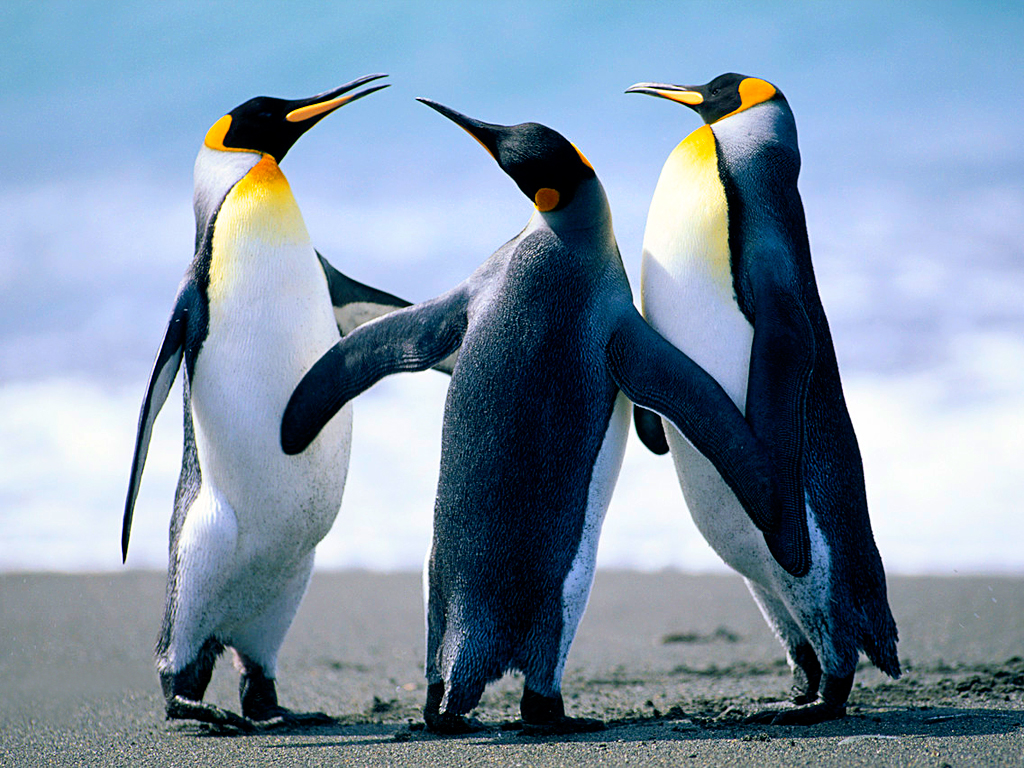
\includegraphics[scale=.50]{figures/Penguins.jpg}
\caption{TAMU figure}
\label{fig:tamu-fig5}
\end{figure}

%%%%%%%%%%%%%%%%%%%%%%%%%%%%%%%%%%%%%%%%%%%%%%%%%%%
%
%  New template code for TAMU Theses and Dissertations starting Fall 2016.
%
%
%  Author: Sean Zachary Roberson 
%	 Version 3.16.09 
%  Last updated 9/12/2016
%
%%%%%%%%%%%%%%%%%%%%%%%%%%%%%%%%%%%%%%%%%%%%%%%%%%%

%%%%%%%%%%%%%%%%%%%%%%%%%%%%%%%%%%%%%%%%%%%%%%%%%%%%%%%%%%%%%%%%%%%%%%
%%                           APPENDIX B
%%%%%%%%%%%%%%%%%%%%%%%%%%%%%%%%%%%%%%%%%%%%%%%%%%%%%%%%%%%%%%%%%%%%%

\chapter{\uppercase {A Second Appendix Whose Title Is Much Longer Than The First}}

Text for the Appendix follows.

\begin{figure}[H]
\centering
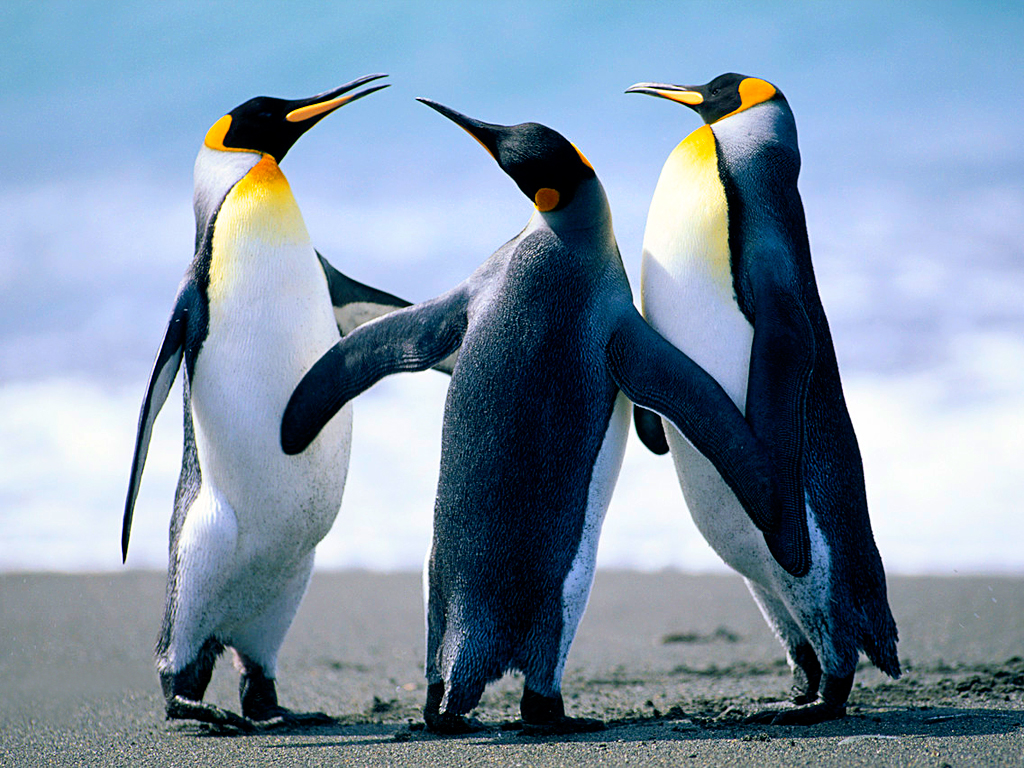
\includegraphics[scale=.50]{figures/Penguins.jpg}
\caption{Another TAMU figure.}
\label{fig:tamu-fig6}
\end{figure}

\section{Appendix Section}

\section{Second Appendix Section}


\pagebreak{}

\end{appendices}


\end{document}
